\documentclass[conference]{IEEEtran}
\usepackage{bm}
\usepackage{cite}
\usepackage{ragged2e}
\usepackage{graphicx}
\usepackage{amsmath}
\usepackage{amssymb}
\usepackage{amsthm}
\usepackage{algorithm}
\usepackage{algpseudocode}
\usepackage{enumitem}
\usepackage{etoolbox}
\usepackage{mathrsfs}
\usepackage{subfig}
\usepackage{array}
\usepackage{cases}
\usepackage{dsfont}
\usepackage{optidef}
\usepackage{cleveref}

\allowdisplaybreaks
\newtheorem{theorem}{Theorem}
\newtheorem{lemma}{Lemma}
\newtheorem{definition}{Definition}
\setlength{\columnsep}{0.21in}
\makeatletter
\newcommand\fs@betterruled{%
  \def\@fs@cfont{\bfseries}\let\@fs@capt\floatc@ruled
  \def\@fs@pre{\vspace*{0.03in}\hrule height.8pt depth0pt \kern2pt}%
  \def\@fs@post{\kern2pt\hrule\relax}%
  \def\@fs@mid{\kern2pt\hrule\kern2pt}%
  \let\@fs@iftopcapt\iftrue}
\floatstyle{betterruled}
\restylefloat{algorithm}
\makeatother
\renewcommand{\arraystretch}{1.2}
\begin{document}
\title{5G DDoS}
\author{\IEEEauthorblockN{Zhan-Lun Chang\IEEEauthorrefmark{1}, Chih-Yu Wang\IEEEauthorrefmark{2}, Hung-Yu Wei\IEEEauthorrefmark{3}}
\IEEEauthorblockA{
\IEEEauthorrefmark{1}\IEEEauthorrefmark{2}Research Center for Information Technology Innovation, Academia Sinica\\
\IEEEauthorrefmark{3}Graduate Institute of Electrical Engineering, National Taiwan University\\
\IEEEauthorrefmark{1}zhc915@citi.sinica.edu.tw,
\IEEEauthorrefmark{2}cywang@citi.sinica.edu.tw,
\IEEEauthorrefmark{3}hywei@ntu.edu.tw,
}}
\maketitle

\begin{abstract}
The network attack such as Distributed Denial-of-Service (DDoS) attack could be critical to latency-critical systems such as Mobile Edge Computing (MEC) as such attacks significantly increase the response delay of the victim service. Intrusion prevention system (IPS) is a promising solution to defend against such attacks, but there will be a trade-off between IPS deployment and application resource reservation as IPS deployment will reduce the number of computation resources for MEC applications. This paper proposed a game-theoretic framework to study the joint computation resource allocation and IPS deployment in the MEC architecture. We study the pricing strategy of the MEC platform operator and purchase strategy of the application service provider, given the expected attack strength and end-user demands. The best responses of both MPO and ASPs are derived theoretically to identify the Stackelberg equilibrium. The simulation results confirm that the proposed solutions significantly increase the social welfare of the system.
\end{abstract}

\section{Introduction}
Mobile edge computing (MEC) is a promising technique to provide low-latency computing services. MEC platform providers (MPOs) deploy MEC servers at the network edge to offer computation resources for latency-critical tasks. Application service providers (ASPs) purchase those resources to deploy their applications for the end-users. This architecture serves as the foundation of 5G/B5G killer applications such as Vehicle Automation, AR/VR, Smart City, etc.

Nevertheless, the network attack has been considered a serious threat to most network services. One of the most common attacks is the Distributed Denial-of-Service (DDoS) attack, in which the attack is performed by many infected devices to send fake requests to the victim service. The service requests of normal end-users will be denied afterward because the victim service is out of resources. We observe that DDoS would be critical in the MEC architecture, as the available resource at the MEC servers are usually limited and cannot be expanded, while the deployed applications are mostly latency-critical and cannot tolerate service denial. A defensive measurement is necessary to guarantee the MEC service quality under the foreseen DDoS attacks.

Intrusion prevention systems (IPS) is an effective measurement to identify and respond to the malicious behaviors performed by the attackers. For instance, in DDoS attacks, an effective IPS instance can recognize those malicious requests and isolate them from the service requests from the normal end-users. Nevertheless, due to the deployment limitation of network edge environment, the candidate IPS for MEC is likely to be software-based, which means there will be a trade-off between IPS deployment and application resource reservation: the deployment of IPS will reduce the amount of computation resource for applications as the IPS instances occupy some, and thus the service latency may increase accordingly. On the other hand, lacking sufficient IPS will make the application vulnerable to DDoS attacks. Such a trade-off should be considered by the ASP when deploying its application at the MEC system. 

In this paper, we proposed a game-theoretic framework to study the joint computation resource allocation and IPS deployment in the MEC architecture from the economic perspective. Specifically, the MPO provides the MEC computation resource in the form of virtual machines with a price. The ASPs buy the VM from the MPO to deploy their applications, and the IPS can be optionally deployed if the DDoS attack is expected. In the proposed framework, we form the problem as a Stackelberg game to study the pricing strategy of the MPO and the optimal amount of VMs for application and IPS deployment of the ASPs. The best responses of both MPO and ASPs are derived theoretically to identify the Stackelberg equilibrium. The simulation results confirm that the proposed solutions significantly increase the social welfare of the system, that is, the total benefit of the whole MEC system.

The main contributions of this work are as follows:
\begin{enumerate}
    \item To the best of our knowledge, we are the first group to study the DDoS attack and defense measurements in the MEC environment in a game-theoretic approach. This approach will help both MPO and ASPs to optimize their configurations in terms of their economic benefits.
    \item We propose a flexible IPS deployment strategy to defend against DDoS attacks at MEC system by allowing ASPs to determine the resource allocation for IPS and main service according to the expected attack strength. 
    \item The optimal strategies of both MPO and ASPs are analyzed through the proposed Stackelberg game model, which can be used to identify the equilibrium in polynomial time. The simulation results verify the effectiveness of the proposed solution in maintaining social welfare. 
\end{enumerate}

This work is based on the previous work \cite{Chang2} but an extended version. We add rigorous proofs in the game formulation part of this paper. We also provide a more precise model to formulate the characteristic of the IPS VM. Moreover, we investigate more complicated cases in the ASP optimization sections. In the MPO optimization section, we proposed a more general case and proof that there are at least one Stackelberg equilibrium. Finally, we use the more realistic parameters in the simulations, and the results gives more illustrations of the model and compare more baseline schemes than the previous work.

\section{Related Works}
Game theory is a powerful tool and can be applied on wireless system, such as resource management \cite{Xu} \cite{Chen2}, power control \cite{Li3} \cite{Zhao}, traffic relaying \cite{Li4}, etc. Game theory also provides a formal framework to solve the optimization problems in MEC orchestration. The Stackelberg game is widely used in many wireless systems \cite{Chang} \cite{Wang2} \cite{Lin2} \cite{Yu}. The matching game is a convenient model to formulate the relationship between the edge servers and mobile users \cite{Liu2} \cite{Lin} \cite{Zhang2}. 

Several studies have been conducted to fight against DDoS attacks.  Alharbi \emph{et al.} introduced NFV and edge computing architecture to design a two-stage DDoS mitigation network\cite{Alharbi}. Mert \emph{et al.}  provided a similar paradigm that security function on edge computing defend the DDoS attack\cite{Mert}. Santoyo-Gonzalez \emph{et al.} presented a lightweight, platform-independent anomaly
detection mechanism based on the BPFabric architecture \cite{Santoyo-Gonzalez}. 

Multi-layer edge framework is another research topic to solve the DDoS problems. Ali \emph{et al.} designed a three-Tier intrusion detection and prevention system in the SDN-IoT environment to assure security \cite{Ali}. A multi-level DDoS mitigation framework \cite{Yan} was proposed by Yan \emph{et al.}  to mitigate the DDoS attack to IoT. Shen \emph{et al.} \cite{Shen} implemented a two-phase DDoS detection system and showed that it could detect attacks with little overhead.

Some papers enhanced intrusion detection with different methods. For example, several articles adopted entropy-based methods to identify the DDoS attack and achieve a decent detection rate\cite{Wang}\cite{Xuanyuan}. Bi \emph{et al.} made use of the feedback of edge routers in the autonomous system to enhance the detection \cite{Bi}. Liu \emph{et al.} developed a Deep Convolution Neural Network Q-learning model to prevent Mirai botnet\cite{Liu}. Zhang \emph{et al.} built dynamic deployment of classifiers based on reinforcement learning model to detect DDoS attacks\cite{Zhang}. FlowGuard, an intelligent edge defense mechanism against IoT DDoS attacks, leveraging long short-term memory (LSTM) and convolutional neural network (CNN) \cite{Jia} was proposed by Jia \emph{et al.} .

Collaborative frameworks also provided a possible solution. Yang \emph{et al.} devised a collaborative task offloading scheme to balance the task load between overloaded and underloaded cloudlets, which can improve the overall performance without additional security frameworks\cite{Yang}. Tan \emph{et al.} used a novel cooperative defense orchestration mechanism and introduced algorithms to effectively organize the cooperation of defense resources in MEC for DDoS mitigation \cite{Tan}. Chen \emph{et al.} proposed a new distributed aggregation scheme and established cooperation among communicating network
domains, which enabled the building of an early warning
system for DDoS defense across multiple internet service provider (ISP) domains \cite{Chen}. Li \emph{et al.} explored the cooperative defense strategy and provided an online cooperative defense framework\cite{Li}. Introduced by Mtibaa \emph{et al.} , detecting and isolating malicious nodes for D2D communication was proposed as another solution to DDoS attacks\cite{Mtibaa}. 

Distinguished from previous works, we focus on the resource allocation problems when defending DDoS attacks. In this paper, we use the Stackelberg game model to formulate
the relationships between MPO and ASPs and solve the subsequent optimization problems to maximize the utility of both sides under the DDoS attacks. 
\section{System Model}\label{sec:system_model}
\begin{figure}[!ht]
\centering
\includegraphics[width= \columnwidth]{5GDDoS_Game_system_architecture.pdf}
\caption{System Architecture}
\label{fig:system}
\end{figure}
We illustrate our system architecture in Fig~\ref{fig:system}. There are three types of entities in our system: the MEC platform operator (MPO), application service providers (ASPs), and end-users (EUs). The MPO manages the computation resources in terms of virtual machines (VMs) of geographically distributed edge servers. Since the ASPs do not have the computation resources to process the application tasks, they have strong demands for the MPO's VMs whose total number is $\mathcal{Q}_{V}$. The goal of the MPO is to maximize its profit by finding the optimal unit selling price $\Psi_{m}^v$ per VM. We denote the set of ASPs as $\mathcal{I}=\{1, \cdots, I\}$. The ASPs determine the number of VMs to buy (denoted by $z_i^v$) from MPO to maximize their profit. The ASPs utilize these purchased VMs to either run the application service or mitigate the DDoS security attacks. If ASPs devote most of their VMs to running the application service, they are prone to DDoS security attacks. The security threat would damage the users' quality of experience (QoE) and thus the revenue of ASPs. Even worse, it would paralyze the application service such that the ASPs have no revenue. On the other hand, if the ASPs devote most of their VMs to mitigating the DDoS attack, they can not ensure good satisfaction to the users (e.g., users' latency requirements can not be satisfied) even though the ASPs are immune from the DDoS attacks. Therefore, it is crucial to find an optimal resource allocation between running the application service and mitigating the DDoS attacks. We denote the set of EUs associated with ASP $i \in \mathcal{I}$ as $\mathrm{U}_i$ and further categorize it into two kinds: normal users (NUs) $\mathrm{U}_i^n$ and malicious users (MUs) $\mathrm{U}_i^m$. Each MU $j \in \mathrm{U}_i$ has the Poisson task arrival rate $\lambda_{ij}$, latency requirement $d_{ij}$, and task size $s_{ij}$. We consider that the EUs do not have enough computation resources or needed resources such as Graphics Processing Unit (GPU) to process the application tasks. Therefore, they will offload the tasks out to the MPO.

The DDoS attacks happen when the AUs flood into the edge servers. The ASPs can intercept some malicious requests by employing open-source intrusion prevention systems (IPS) such as Suricata \cite{Suricata}. The IPS of all ASPs monitors and filters all task requests, and all VMs devoted to running the application service process the filtered task requests. We assume the IPS does not classify the normal task requests as malicious, but it can not discern all malicious requests and would classify some malicious task requests as normal. How many malicious requests can the IPS filter depends on how many VMs the ASPs dedicate to the IPS. We use $H(\cdot)$ to represent the relationship between the quantity of intercepted malicious requests and the number of devoted VMs. $H(\cdot)$ is assumed to be non-decreasing and concave. Also, $H(0)=0$.

We consider orthogonal frequency-division multiple access (OFDMA) system and thus the bandwidth of the edge servers whose computation resources are allocated to ASP $i$ denoted by $B_i$ can be divided into $|\mathrm{U}_i|$ sub-bands of size $W_{i} = B_i/|\mathrm{U}_i|$. Each MU $j\in \mathrm{U}_i$ transmits the data over each of $|\mathrm{U}_i|$ sub-bands, and hence they would not cause interference to other EUs while transmitting. The maximum achievable uplink data transmission rate $R_{ij}$ between ASP $i$ and MU $j \in \mathrm{U}_i$ is
\begin{equation} \label{eqn:shannon}
R_{ij}=W_i \cdot log_2\Big(1+\frac{p_{ij}g_{ij}}{N_{0}}\Big)
\end{equation}
where $p_{ij}$ is the maximum transmission power of MU $j$ in $\mathrm{U}_i$, and $g_{ij}$ denotes the uplink channel gain between ASP $i$ and MU $j$. $N_0$ is the background noise power. Based on this rate, we can calculate the mean transmission time of workload consisting of tasks with size $s_{ij}$ from MU $j \in \mathrm{U}_i$ to ASP $i$.
\begin{equation}
T_{ij}^t=\frac{\lambda_{ij} \cdot s_{ij}}{R_{ij}}
\end{equation}

The task arrival process at ASP $i$ still follows the Poisson process according to the Poisson process's stationary property. Furthermore, the mean arriving rate of the Poisson process at ASP $i$ can be expressed as $\lambda_i = \sum_{j \in \mathrm{U}_i} \lambda_{ij}$ based on the superposition property of the Poisson process. Moreover, we use $\lambda_i^m$ to indicate the total arrival rate of malicious request, which is expressed as $\lambda_i^m = \sum_{j \in \mathrm{U}_i^m} \lambda_{ij}$. Similarly, we can also define the total arrival rate of normal request as $\lambda_i^n$, where $\lambda_i^n =  \sum_{j \in \mathrm{U}_i^n} \lambda_{ij}$. Since the ASPs buy VMs from MPO whose overall computation resources are still limited compared to the cloud platform such as Google cloud platform or Amazon EC2 platform, we model the meaning processing delay of all VMs purchased by ASPs using $M/M/1$ queue. Each VM of MPO is homogeneous and can process $f_m^v$ CPU cycles per second. As the average required CPU cycles for a task of ASP $i$ may be different, the mean service rate of the queue at ASP $i$ denoted by $\mu_i^v$ (the number of tasks that a VM can process on average per second) is different for every ASP $i$. We denote the required CPU cycles of user $j \in \mathsf{U}_i$ as $\chi_{ij}$. The relationship between $f_m^v$ and $\mu_i^v$ is
\begin{equation}\label{eqn:service_rate}
\mu_i^v = f_m^v/(\frac{\sum_{j \in \mathsf{U}_i} \chi_{ij}}{|\mathrm{U}_i|})
\end{equation}
If the ASP $i$ devotes $z_i^h$ out of $z_i^v$ VMs to IPS, the intercepted quantity of malicious requests is $H_i(z_i^h)$. When ASP $i$ buys $z_i^v$ VMs from the MPO and devotes $z_i^h$ to IPS, those VMs' mean processing delay is
\begin{equation} \label{eqn:asp_mm1_delay}
T_i^p(z_i^v, z_i^h) = \frac{1}{(z_i^v - z_i^h)\mu_i^v - \big(\lambda_i - H_i(z_i^h)\big)}
\end{equation}
Under the condition that all malicious requests are intercepted, the ASP cannot intercept more malicious requests by deploying more IPS VMs. Therefore, the value of $H_i(x)$ reaches the quantity of malicious requests and remains this maximal value when $x$ is larger than certain value. In this paper, we consider the function of the ASP $i$ with a linear form of
\begin{equation}
\begin{aligned}
    H_i(x) = min(\eta{x}, \lambda_i^m)
\end{aligned}
\end{equation}
so that the closed form solutions can be derived in the following optimization problems, and $\lambda_i^m$ indicates the total quantity of malicious requests of ASP $i$. The cost of using IPS only comes from the devoted VMs and does not include any payment because it is open-source.

The payment from the NU $j \in \mathrm{U}_i^n$ to the ASP $i$ depends on whether the latency requirements $d_{ij} \, \forall j \in \mathrm{U}_i^n$ are satisfied or not. If latency requirements $d_{ij}$ are met, NU $j \in \mathrm{U}_i^n$ pays a price $\Psi_{ij}$ to ASP $i$. The heterogeneity of the payment reflects the different characteristics of NUs. The NUs with different latency requirements may have different level of satisfaction with the same service provided by the ASP $i$. If latency requirements $d_{ij}$ are not met, NU $j \in \mathrm{U}_i^n$ does not pay ASP $i$. The MUs $j \in \mathrm{U}_i^m$ will not pay any money to the ASP $i$ no matter whether their latency requirement are satisfied or not. We represent the payment of EU $j \in \mathrm{U}_i$ as follows:
\begin{subnumcases}{\mathcal{K}_{ij}(z_i^v, z_i^h)=\label{eqn:devicepayment}}
  \Psi_{ij} & \hspace*{-1.7mm}if $T_{ij}^t + T_i^p(z_i^v, z_i^h) \leq d_{ij}$, $j \in \mathrm{U}_i^n$\\
  0 & \hspace*{-1.7mm}if $T_{ij}^t + T_i^p(z_i^v, z_i^h) > d_{ij}$, $j \in \mathrm{U}_i^n$ \\
  0 & \hspace*{-1.7mm}$j \in \mathrm{U}_i^m$
\end{subnumcases}

\section{Game Formulation}\label{sec:game_formulations}
Because of the rationalities of both MPO and ASPs, the intrinsic hierarchy between MPO and ASPs, and the influence of one ASP's action on other ASPs' profits, we model the interaction between MPO and ASPs as a two-stage single-leader-multi-followers Stackelberg game. Both the MPO and ASPs are rational players and have the ultimate goal of maximizing their profits by adjusting their actions. The MPO can select a price per VM $\Psi_{m}^v$ that maximizes its profit, and the ASPs determine how many VMs to buy from MPO $z_i^v \, \forall i$ to optimize its profit too. The MPO's selection of price per VM affects how many VMs those ASPs would buy, which impacts the choice of price. Since the ASPs need to buy the computation resources from MPO to maintain their application services, the MPO has an advantage over the ASPs.
Moreover, due to MPO's finite number of VMs, the more one ASP buys, the less other ASPs can buy. The action of one ASP affects other ASPs' profit. The Stackelberg game where the MPO acts as the leader and all ASPs are the followers can capture the coupled and hierarchical relationship between MPO and ASPs, the self-interests of both MPO and ASPs, and the implicit influence among ASPs. We illustrate the actions and utilities of MPO and ASPs in the following first and then formulate the optimization problems for both players.

\subsection{The Action and The Utility of ASPs}
Given the MPO's price per VM $\Psi_m^v$, each ASP $i$ chooses how many VMs to buy from the MPO $z_i^v$ to maximize its profit which is the revenue accrued from the normal MU $j \in \mathrm{U}_i^n$ minus the payment to the MPO for purchasing $z_i^v$ VMs. The natural candidate for the utility is the profit. However, even with the same $z_i^v$, the revenue of ASP $i$ hinges on how many VMs it dedicates to the IPS, distribution of latency requirements $d_{ij}$, and the different payments of heterogeneous NU $j \in \mathrm{U}_i^n$. We define the utility of ASP $i$ when it purchases $z_i^v$ VMs from MPO as the maximum expected profit across the different number of VMs dedicates to the IPS $z_i^h$ with respect to the distribution of latency requirement $d_{ij}$. Furthermore, to make the optimization problem tractable, we assume that the latency requirements $d_{ij} \, \forall j \in \mathrm{U}_i$ are drawn from the same uniform distribution indexed by $i$ over interval $[a_i, b_i]$ denoted by $\mathcal{U}(a_i,b_i)$ and relax the variables of ASPs $z_i^v, z_i^h \, \forall i \in \mathcal{I}$ to real numbers. The utility of ASP $i$ given $\Psi_m^v$ is
\begin{align}
&Y_i(z_i^v|\Psi_m^v) \triangleq \max_{z_i^h} \mathsf{E}_{d_{ij}}\Big[\sum_{j \in \mathrm{U}_i^n} \mathcal{K}_{ij}(z_i^v, z_i^h) - \Psi_m^v z_i^v\Big] \\
&\hspace*{-1mm}=\max_{z_i^h} \mathsf{E}_{d_{ij}}[\sum_{j \in \mathrm{U}_i^n}\Psi_{ij}\mathds{1}\{T_{ij}^t + T_i^p(z_i^v, z_i^h) \leq d_{ij}\} - \Psi_m^vz_i^v] \nonumber \\
&\hspace*{-1mm}=\max_{z_i^h} [\sum_{j \in \mathrm{U}_i^n}\Psi_{ij}(1-F_{d_{ij}}(T_{ij}^t+T_i^p(z_i^v, z_i^h)) - \Psi_m^vz_i^v] \label{eqn:asp_def_subobjective_unfold} \\
&\hspace*{-1mm}\triangleq \max_{z_i^h} X_i(z_i^h|z_i^v,\Psi_m^v) \label{eqn:asp_def_subobjective}
\end{align}
where the $F_{X}(x)$ is the cumulative distribution function (CDF) of $\mathcal{U}(a_i,b_i)$ and its definition is shown as
\begin{subnumcases}{F_X(x)=\label{eqn:CDF}}
  0 & $x < a_i$\\
  \frac{x-a_i}{b_i-a_i} &  $x \in[a_i, b_i]$\\
  1 & $x > b_i$
\end{subnumcases}

$\mathsf{E}_{d_{ij}}$ means taking expectation with respect to the distribution of $d_{ij}$, and $\mathds{1}\{\cdot\}$ is the indicator function. $F_{d_{ij}}(T_{ij}^t+T_i^p(z_i^v, z_i^h))$ is the probability that the latency requirement $d_{ij}$ of the NU $j\in\mathrm{U}_i^n$ are not satisfied, which is also the CDF of $\mathcal{U}(a_i,b_i)$. Given $z_i^v$, we have two constraints on $z_i^h$. First, the number of VMs dedicated to IPS $z_i^h$ must be no larger than the number of purchased VMs $z_i^v$. Second, to make the processing queue stable, the mean service rate by the VMs dedicated to running the service must be higher than the mean arrival rate for EUs $j \in \mathrm{U}_i$. To define the utility of ASP $i$ when the purchased VMs from the MPO is $z_i^v$, we have to solve the following optimization problem.
\begin{maxi!}[2]
  {z_i^h \in \mathbb{R}}
  {X_i(z_i^h|z_i^v,\Psi_m^v) \label{eqn:asp_utility_def_opti_obj}}
  {\label{eqn:asp_utility_def_opti}}
  {}
  \addConstraint{0 \leq z_i^h \leq \xi_i z_i^v}{\label{eqn:asp_utility_def_opti_const1}}
  \addConstraint{0 < (z_i^v-z_i^h)\mu_i^v - \lambda_i + H_i(z_i^h) }{\label{eqn:asp_utility_def_opti_const2}}
\end{maxi!}
In (\ref{eqn:asp_utility_def_opti_const1}), we further introduce a system parameter $\xi_i\in[0, 1]$ to control the feasible range of $z_i^h$.
The observation that both (\ref{eqn:asp_utility_def_opti_const1}) and (\ref{eqn:asp_utility_def_opti_const2}) impose upper bounds on the range of $z_i^h$ will simplify the characterization of the optimal $z_i^h$. Showing the utility of the ASP $i$, $Y_i(z_i^v)$, is well-defined is equivalent to proving the optimization problem (\ref{eqn:asp_utility_def_opti}) has at lease one solution. If there are multiple optimal points that have the same values of $X_i(z_i^h|z_i^v,\Psi_m^v)$, we randomly select one to be the solution to (\ref{eqn:asp_utility_def_opti}).

Otherwise, we can rewrite the term $\sum_{j \in \mathrm{U}_i^n}\Psi_{ij}(1-F_{d_{ij}}(T_{ij}^t+T_i^p(z_i^v, z_i^h))$ using the definition of $F_{d_{ij}}(T_{ij}^t+T_i^p(z_i^v, z_i^h))$, so it becomes\footnote{In the rest of the paper, we assume that the $T_{ij}^t+T_i^p(z_i^v, z_i^h)$ lies in the range of $[a_i, b_i]$, so we assume $\mathrm{U}_i^{n2} = \mathrm{U}_i^{n}$.}
\begin{equation}
\begin{aligned}
&\sum_{j \in \mathrm{U}_i^{n1}}\Psi_{ij} \times 1 +\sum_{j \in \mathrm{U}_i^{n2}}\Psi_{ij} \times (1-\frac{T_{ij}^t+T_i^p(z_i^v, z_i^h)-a_i}{b_i-a_i})+\\
&\sum_{j \in \mathrm{U}_i^{n3}}\Psi_{ij} \times 0
\end{aligned}
\end{equation}
, where we divide $\mathrm{U}_i^{n}$ into three sets $\mathrm{U}_i^{n1}$, $\mathrm{U}_i^{n2}$ and $\mathrm{U}_i^{n3}$.
We define these three sets as 
\begin{subequations}\label{normal_set_user}
\begin{align}
\mathrm{U}_i^{n1} =& \{T_{ij}^t+T_i^p(z_i^v, z_i^h) < a_i\ |\ j \in \mathrm{U}_i^{n}\}\label{normal_set_user_1} \\
\mathrm{U}_i^{n2} =& \{a_i \leq T_{ij}^t+T_i^p(z_i^v, z_i^h) \leq b_i\ |\ j \in \mathrm{U}_i^{n}\}\label{normal_set_user_2} \\
\mathrm{U}_i^{n3} =& \{ b_i < T_{ij}^t+T_i^p(z_i^v, z_i^h) \ |\ j \in \mathrm{U}_i^{n}\}\label{normal_set_user_3}
\end{align}
\end{subequations}
\begin{lemma}
The utility of ASP $i$, $Y_i(z_i^v)$, is well defined. That is, the optimization problem (\ref{eqn:asp_utility_def_opti}) has at least one optimal point. Moreover, the optimization problem (\ref{eqn:asp_utility_def_opti}) is a convex optimization problem.
\end{lemma}
\begin{proof}
The feasible region imposed by (\ref{eqn:asp_utility_def_opti_const1}) and (\ref{eqn:asp_utility_def_opti_const2}) is a closed and bounded interval in $\mathbb{R}$ and thus is a convex set. As the objective function (\ref{eqn:asp_utility_def_opti_obj}) is continuous in $z_i^h$, the existence of the optimal solution then comes from the Extreme Value Theorem. If (\ref{eqn:asp_utility_def_opti_obj}) is concave at each feasible $z_i^h$, optimization problem (\ref{eqn:asp_utility_def_opti}) is a convex optimization problem. It remains to show that the objective function (\ref{eqn:asp_utility_def_opti_obj}) is concave in feasible $z_i^h$. By rearranging the terms, we express $X_i(z_i^h|z_i^v,\Psi_m^v)$ as
\begin{equation}
\begin{aligned}
    \sum_{j \in \mathrm{U}_i^{n}}\Psi_{ij}(1-\frac{T_{ij}^t+T_i^p(z_i^v, z_i^h)-a_i}{b_i-a_i})- \Psi_m^v z_i^v 
\end{aligned}
\end{equation}
To show $X_i(z_i^h|z_i^v,\Psi_m^v)$ is concave in feasible $z_i^h$, it suffices to show that $T_i^p(z_i^v, z_i^h)$ is convex in feasible $z_i^h$. We will verify the convexity of $T_i^p(z_i^v, z_i^h)$. From (\ref{eqn:asp_mm1_delay}), We can rewrite it as
\begin{equation} 
\begin{aligned}
T_i^p(z_i^v)=\frac{1}{(z_i^v-z_i^h)\mu_i^v - \lambda_i + H_i(z_i^h)}
\end{aligned}
\end{equation}
By definition, $H_i(z_i^h)$ is concave in feasible $z_i^h$. In addition, $(z_i^v-z_i^h)\mu_i^v - \lambda_i$ is an affine function of $z_i^h$, so $(z_i^v-z_i^h)\mu_i^v - \lambda_i + H_i(z_i^h)$ is concave in feasible $z_i^h$.

Given a positive concave function $f(x)$ in feasible $x$, $\frac{1}{f(x)}$ is convex in feasible $x$\cite[Chapter~3.2]{boyd2004convex}. Therefore, $T_i^p(z_i^v, z_i^h)$ is convex in feasible $z_i^h$ and $X_i(z_i^h|z_i^v,\Psi_m^v)$ is concave in feasible $z_i^h$.
\end{proof}

After defining the utility of ASP $i$, $Y_i(z_i^v)$, we can now formulate the optimization problem of ASP $i$ given the MPO's price per VM $\Psi_m^v$.
\begin{maxi!}[2]
  {z_i^v \in \mathbb{R}}
  {Y_i(z_i^v|\Psi_m^v) \label{eqn:asp_utility_opti_obj}}
  {\label{eqn:asp_utility_opti}}
  {}
  \addConstraint{\lambda_i+ \gamma_i \leq z_i^v \mu_i^v}{\label{eqn:asp_utility_opti_const1}}
  \addConstraint{0 \leq Y_i(z_i^v|\Psi_m^v)}{\label{eqn:asp_utility_opti_const2}}
\end{maxi!}
The constraint (\ref{eqn:asp_utility_opti_const1}) regulates that when the ASP $i$ dedicates all purchased VMs to running the application service, the mean service rate must be larger than the mean arrival rate by at least $\gamma_i$, where $\gamma_i\geq 0$. (\ref{eqn:asp_utility_opti_const1}) also ensures that the feasible region of (\ref{eqn:asp_utility_def_opti}) is non-empty because under this constraint, there is at least one $z_i^h$ that satisfies (\ref{eqn:asp_utility_def_opti_const2}). The constraint (\ref{eqn:asp_utility_opti_const2}) represents the individual rationality for every ASP. That is, when making the processing queue stable gives a negative utility, the ASPs would rather choose not to serve the users' requests and do not buy any VMs from the MPO, which has zero utility. We defer the analysis of solutions to both optimization problems (\ref{eqn:asp_utility_def_opti}) and (\ref{eqn:asp_utility_opti}) to the \Cref{sec:game_optimization}. We denote the solution to (\ref{eqn:asp_utility_opti}) as $(z_i^v(\Psi_m^v))^*$ to emphasize the dependence on the MPO's price per VM $\Psi_m^v$.

\subsection{The Action and The Utility of The MPO}
With the prediction about the number of VMs purchased by ASPs $(z_i^v(\Psi_m^v))^* \, \forall i \in \mathcal{I}$, the MPO chooses the price per VM $\Psi_m^v$ to maximize its utility which is defined as the MPO's profit. The revenue of the MPO is the sum of payments from all ASPs. Although the ASPs buy the VMs from the MPO, it is the infrastructure of the MPO that processes the application requests. As a result, the MPO has an operating cost for keeping the VMs working. We represent the cost for operating $\sum_{i \in \mathcal{I}} (z_i^v(\Psi_m^v))^*$ VMs by $C_m^v\big(\sum_{i \in \mathcal{I}} (z_i^v(\Psi_m^v))^*\big)$. The function $C_m^v(\cdot)$ is assumed to be convex and non-decreasing, which means that both the marginal cost and the cost increase as the number of VMs that the MPO has to keep running increases. We denote the MPO's utility as $Y_m(\Psi_m^v)$ and formulate the MPO's optimization problem.
\begin{maxi!}[2]
  {\Psi_m^v}
  {\Psi_m^v \cdot \sum_{i \in \mathcal{I}} (z_i^v(\Psi_m^v))^* - C_m^v\big(\sum_{i \in \mathcal{I}} (z_i^v(\Psi_m^v))^*\big) \label{eqn:mpo_utility_opti_obj}}
  {\label{eqn:mpo_utility_opti}}
  {}
  \addConstraint{\sum_{i \in \mathcal{I}} (z_i^v(\Psi_m^v))^* \leq \mathcal{Q}_v}{\label{eqn:mpo_utility_opti_const1}}
  \addConstraint{0 \leq \Psi_m^v}{\label{eqn:mpo_utility_opti_const2}}
\end{maxi!}
The constraint (\ref{eqn:mpo_utility_opti_const1}) mandates that the MPO can not sell more VMs than the total number of VMs $\mathcal{Q}_v$ that the MPO has. The constraint (\ref{eqn:mpo_utility_opti_const1}) imposes a lower bound for MPO's price per VM. The constraint (\ref{eqn:mpo_utility_opti_const2}) requires the MPO's price per VM must be non-negative. The property of this optimization (\ref{eqn:mpo_utility_opti}) relies on the solution $(z_i^v(\Psi_m^v))^*$, and we defer the analysis to \Cref{sec:game_optimization}.
\section{Game Optimization} \label{sec:game_optimization}
We would leverage the backward induction principle to solve the formulated Stackelberg game. In this principle, we solve the followers' (ASPs') optimization problems first and then the leader's (the MPO's) optimization problem based on responses of ASPs to the MPO's price per VM, i.e., $(z_i^v(\Psi_m^v))^* \, \forall i \in \mathcal{I}$. Before delving into the solution process, we first define the Stackelberg game equilibrium. We symbolize the ASP $i$'s action set using $\mathcal{A}_i$ and the profile of all ASPs' action using $\bm{z^v}=(z_1^v, z_2^v, \cdots, z_I^v) \in \mathcal{A}_1 \times \mathcal{A}_2 \cdots \times \mathcal{A}_I$ where $\mathcal{A}_1 \times \mathcal{A}_2$ means the Cartesian product of $\mathcal{A}_1$ and $\mathcal{A}_2$. The ASP $i$'s best response set $\mathcal{B}_i^R(\Psi_m^v)$ to the MPO's price per VM $\Psi_m^v$ is given by
\begin{equation} \label{eqn:asp_best_response}
\begin{aligned}
\mathcal{B}_i^R(\Psi_m^v) = &\{z_i^v \in \mathcal{A}_i |Y_i(z_i^v|\Psi_m^v) \geq Y_i\big((z_i^v)'|\Psi_m^v\big) \\
&\forall (z_i^v)' \in \mathcal{A}_i, (z_i^v)' \neq z_i^v\}
\end{aligned}
\end{equation}
We also denote the Cartesian product of all ASPs' best response sets as
\begin{equation}
\mathcal{B}^R(\Psi_m^v) = \mathcal{B}_1^R(\Psi_m^v) \times \mathcal{B}_2^R(\Psi_m^v) \cdots \times \mathcal{B}_I^R(\Psi_m^v)
\end{equation}
Likewise, we denote the MPO's action set as $\mathcal{A}_m$. Furthermore, to stress the influence of ASPs' actions on the MPO's utility, we use $Y_m(\Psi_m^v|\bm{z^v})$ to represent the MPO's utility in the following definition of the MPO's best response set.
\begin{equation} \label{eqn:mpo_best_response}
\begin{aligned}
\mathcal{B}_m = &\{\Psi_m^v \in \mathcal{A}_m| Y_m(\Psi_m^v|\bm{z^v}) \geq Y_m((\Psi_m^v)'|(\bm{z^v})') \\
&\forall (\Psi_m^v)' \in \mathcal{A}_m, (\Psi_m^v)' \neq \Psi_m^v, \forall \bm{z^v} \in \mathcal{B}^R(\Psi_m^v) \\
&\forall  (\bm{z^v})' \in \mathcal{B}^R\big((\Psi_m^v)'\big)\}
\end{aligned}
\end{equation}
\begin{definition}[\textbf{Stackelberg equilibrium}] \label{def:stackelberg_equilibrium}
If $\mathcal{B}_{m}$ and $\mathcal{B}^R(\Psi_m^v)$ are both non-empty, the Stackelberg equilibrium in our mechanism is a vector of dimension $(I+1)$ that is an element of $\mathcal{B}_m  \times \mathcal{B}^R(\Psi_m^v)$.
\end{definition}
We analyze the solution process of the formulated Stackelberg game according to whether the solution to (\ref{eqn:asp_utility_def_opti}) is the extreme point or boundary point of the constraint.
\begin{figure}[!ht]
    \centering
    \includegraphics[width=\columnwidth]{5GDDoS_Game_Flow_Chart.pdf}
    \caption{Flow Chart of the Solution Process}
    \label{fig:flow_chart}
\end{figure}
\subsection{ASP Optimization Problem}
\textbf{Case 1}: The optimal point of (\ref{eqn:asp_utility_def_opti}) is the extreme point whose first derivative with respect to $z_i^h$. The first derivative of $X_i(z_i^h|z_i^v,\Psi_m^v)$ with respect to $z_i^h$ is
\begin{equation} \label{eqn:asp_utilitu_def_firstderiv}
[(z_i^v - z_i^h) - \lambda_i + H_i(z_i^h)]^{-2} \cdot (-\mu_i^v + H_i'(z_i^h))
\end{equation}
% $(z_i^v - z_i^h) - \lambda_i + H_i(z_i^h)$ is positive at every feasible $z_i^h$ because of the constraint (\ref{eqn:asp_utility_def_opti_const2}). Also, $H'(\cdot)$ is non-decreasing and thus has an inverse function denoted by $G(\cdot)$. We can solve the extreme point denoted by $(z_i^h)^*$ through letting (\ref{eqn:asp_utilitu_def_firstderiv}) equal zero.
% \begin{equation} \label{eqn:asp_utility_def_extreme_point}
% (z_i^h)^* = (H')^{-1}(\mu_i^v) \triangleq G(\mu_i^v)
% \end{equation}
% When we substitute (\ref{eqn:asp_utility_def_extreme_point}) into (\ref{eqn:asp_mm1_delay}), the mean processing delay denoted as $T_{i,1}^p(z_i^v)$ depends only on $z_i^v$ and is
% \begin{equation}
% T_{i,1}^p(z_i^v) = \frac{1}{\big(z_i^v - G(\mu_i^v)\big)\mu_i^v - \lambda_i + H\big(G(\mu_i^v)\big)}
% \end{equation}
% According to (\ref{eqn:asp_def_subobjective_unfold}) and (\ref{eqn:asp_def_subobjective}), the objective function (\ref{eqn:asp_utility_opti_obj}) becomes
% \begin{equation}\label{eqn:asp_case1_utility}
% \begin{aligned}
% Y_i^1(z_i^v|\Psi_m^v) \triangleq \sum_{j \in \mathrm{U}_i^{n}}\Psi_{ij}(1-\frac{T_{ij}^t + T_{i,1}^p(z_i^v)-a_i}{b_i-a_i}) - \Psi_m^vz_i^v
% \end{aligned}
% \end{equation}
% If we optimize (\ref{eqn:asp_case1_utility}), we can observe how the ASP reacts to different $z_i^v$ and $\Psi_m^v$ in order to reach the highest utility. 

However, we won't try to do so since the case doesn't happen based on the initial assumption of $H_i(x) = min(\eta{x}, \lambda_i^m)$. We explain the property in the following.
\begin{lemma} \label{lemma:asp_case1_not_exist}
$X_i(z_i^h|z_i^v,\Psi_m^v)$ doesn't have extreme point in feasible $z_i^h$ if $H_i(x) = min(\eta{x}, \lambda_i^m)$.
\end{lemma}
\begin{proof}
From (\ref{eqn:asp_utilitu_def_firstderiv}),  we substitute $\eta{z_i^h}$ into $H_i(z_i^h)$, then we can obtain
\begin{equation} \label{eqn:asp_utilitu_simplified}
[(z_i^v - z_i^h) - \lambda_i + \eta{z_i^h}]^{-2} \cdot (-\mu_i^v + \eta)
\end{equation}
Obviously, no matter what the value of $z_i^h$ is, (\ref{eqn:asp_utilitu_simplified}) equaling zero will never be satisfied. Therefore, the extreme point does not exist.\qedhere
\end{proof}
Now we know that the extreme point of (\ref{eqn:asp_utility_def_opti_obj}) does not exist in feasible $z_i^h$, so the maximum value of $X_i(z_i^h|z_i^v,\Psi_m^v)$ only happens at the boundary points of feasible $z_i^h$. Moreover, for linear form of $H_i(x)$, the coefficient $\eta$ indicates the efficiency of the IPS VM. If the efficiency of the IPS VM $\eta$ is larger than the service rate $\mu_i^v$, the ASP would tend to deploy as much IPS ratio as it could. In contrast, if the efficiency of the IPS VM $\eta$ is smaller than the service rate $\mu_i^v$, the ASP would tend to serve its users instead of intercepting malicious requests. 

\textbf{Case 2}: In this case, the efficiency of the IPS VM $\eta$ is larger than the service rate $\mu_i^v$ of the ASP $i$. Therefore, the ASP has more incentive to deploy as many IPS VM as they could. In this situation, the optimal point of (\ref{eqn:asp_utility_def_opti}) is the right boundary of (\ref{eqn:asp_utility_def_opti_const1}) or the exact number of VM required to defend all of the malicious requests. That is, with a specific form of $H_i(x) = min(\eta x, \lambda_i^m)$ and the purchased number of VM is $z_i^v$, the ASP $i$'s optimal number of VMs devoted to the IPS is
\begin{equation} \label{eqn:asp_utility_def_first_boundary}
(z_i^h)^* = min(\xi_i z_i^v, \frac{\lambda_i^m}{\eta})
\end{equation}

We substitute $(z_i^h)^*$ into (\ref{eqn:asp_mm1_delay}), the mean processing delay in this case denoted as $T_{i,2}^p(z_i^v)$ is

\begin{subnumcases}{=\label{eqn:asp_case2_mm1_delay}}
  \frac{1}{(1-\xi_i)z_i^v\mu_i^v - \big(\lambda_i - \eta \xi_iz_i^v\big)} & $z_i^v<\frac{\lambda_i^m}{\eta \xi_i}$ \label{eqn:asp_case2_mm1_delay1} \\
  \frac{1}{(z_i^v-\frac{\lambda_i^m}{\eta})\mu_i^v - \big(\lambda_i - \lambda_i^m\big)} & $z_i^v\geq\frac{\lambda_i^m}{\eta \xi_i}$ \label{eqn:asp_case2_mm1_delay2}
\end{subnumcases}

According to (\ref{eqn:asp_def_subobjective_unfold}) and (\ref{eqn:asp_def_subobjective}), the objective function (\ref{eqn:asp_utility_opti_obj}) becomes
\begin{equation} \label{eqn:asp_case2_objective}
\begin{aligned}
Y_i^2(z_i^v|\Psi_m^v) \triangleq \sum_{j \in \mathrm{U}_i^{n}}\Psi_{ij}(1-\frac{T_{ij}^t + T_{i,2}^p(z_i^v)-a_i}{b_i-a_i}) - \Psi_m^vz_i^v
\end{aligned}
\end{equation}
If $Y_i^2(z_i^v|\Psi_m^v)$ is concave in feasible $z_i^v$, it is much easier to solve the optimization problem (\ref{eqn:asp_utility_opti}) with the objective being $Y_i^2(z_i^v|\Psi_m^v)$. We prove this properties in the following.
\begin{lemma} \label{lemma:asp_case2_utility_concave}
$Y_i^2(z_i^v|\Psi_m^v)$ is concave in feasible $z_i^v$.
\end{lemma}
\begin{proof}
If $T_{i,2}^p(z_i^v)$ is convex in feasible $z_i^v$, $Y_i^2(z_i^v|\Psi_m^v)$ is concave in feasible $z_i^v$. We will verify the convexity of $T_{i,2}^p(z_i^v)$. We can write $T_{i,2}^p(z_i^v)$ as follow
\begin{equation} \label{eqn:asp_case2_mm1_delay_min}
\begin{aligned}
\frac{1}{(z_i^v-min(\xi_i z_i^v, \frac{\lambda_i^m}{\eta}))\mu_i^v - \big(\lambda_i - \eta\min(\xi_i z_i^v, \frac{\lambda_i^m}{\eta})\big)}
\end{aligned}
\end{equation}
By rewriting (\ref{eqn:asp_case2_mm1_delay_min}), $T_{i,2}^p(z_i^v)$ can be further expressed as
\begin{equation} \label{eqn:asp_case2_mm1_delay_min_new}
\begin{aligned}
T_{i,2}^p(z_i^v) = \frac{1}{z_i^v\mu_i^v - \lambda_i +(\eta - \mu_i^v)\min(\xi_i z_i^v, \frac{\lambda_i^m}{\eta})}
\end{aligned}
\end{equation}
Since the term $(\eta - \mu_i^v)$ is always positive in Case 2, $(\mu_i^v - \eta)\min(\xi_i z_i^v, \frac{\lambda_i^m}{\eta})$ is positive and concave in feasible $z_i^v$. In addition, $(z_i^v\mu_i^v - \lambda_i)$ is an affine function in feasible $z_i^v$, so $z_i^v\mu_i^v - \lambda_i+(\mu_i^v - \eta)\min(\xi_i z_i^v, \frac{\lambda_i^m}{\eta})$ is concave in feasible $z_i^v$\cite[Chapter~3.2]{boyd2004convex}.

Given a concave function $f(x)$ in feasible $x$, $\frac{1}{f(x)}$ is convex in feasible $x$. Therefore, $T_{i,2}^p(z_i^v)$ is convex in feasible $z_i^v$ and $Y_i^2(z_i^v|\Psi_m^v)$ is concave in feasible $z_i^v$.  \qedhere
\iffalse
% If $z_i^v < \frac{\lambda_i^m}{\eta \xi_i}$, the second derivative of
% $T_{i,2}^p(z_i^v)$ with respect to $z_i^v$ is
% \begin{equation} \label{eqn:asp_case2_mm1_delay_second_deriv1}
% \begin{aligned}
% &2[(1-\xi_i)\mu_i^v z_i^v - \lambda_i + H_i(\xi_i z_i^v)]^{-3}\times [(1-\xi_i)\mu_i^v\\
% &+ \xi_i H'(\xi_i z_i^v)]^2-[(1-\xi_i)\mu_i^v z_i^v - \lambda_i + H_i(\xi_i z_i^v)]^{-2}  \\
% & \times (\xi_i)^2 H''(\xi_i z_i^v)
% \end{aligned}
% \end{equation}
% Since $(z_i^h)^* = \xi_i z_i^v$ satisfies the constraint (\ref{eqn:asp_utility_def_opti_const2}), $(1-\xi_i)\mu_i^v z_i^v - \lambda_i + H_i(\xi_i z_i^v)$ is always positive. Moreover, as $H_i(\cdot)$ is concave, $H''(\xi_i z_i^v)$ is non-positive. The first term of (\ref{eqn:asp_case2_mm1_delay_second_deriv1}) is positive, and the second term of (\ref{eqn:asp_case2_mm1_delay_second_deriv1}) is non-positive. Therefore, (\ref{eqn:asp_case2_mm1_delay_second_deriv1}) is non-negative.

% If $z_i^v > \frac{\lambda_i^m}{\eta \xi_i}$, the second derivative of $T_{i,2}^p(z_i^v)$ with respect to $z_i^v$ is
% \begin{equation} \label{eqn:asp_case2_mm1_delay_second_deriv2}
% \begin{aligned}
% &2[(z_i^v-\frac{\lambda_i^m}{\eta})\mu_i^v  - \lambda_i + \lambda_i^m]^{-3}\times (\mu_i^v)^2
% \end{aligned}{}
% \end{equation}
% Since $(z_i^h)^* = \frac{\lambda_i^m}{\eta}$ satisfies the constraint (\ref{eqn:asp_utility_def_opti_const2}), $(z_i^v-\frac{\lambda_i^m}{\eta})\mu_i^v  - \lambda_i + \lambda_i^m$ is always positive. Moreover, as $(\mu_i^v)^2$ is non-negative,  (\ref{eqn:asp_case2_mm1_delay_second_deriv2}) is positive. Therefore, (\ref{eqn:asp_case2_mm1_delay_second_deriv2}) is non-negative.

% Both (\ref{eqn:asp_case2_mm1_delay_second_deriv1}) and (\ref{eqn:asp_case2_mm1_delay_second_deriv2}) are non-negative, which means $T_{i,2}^p(z_i^v)$ is convex in feasible $z_i^v$. Hence, $Y_i^2(z_i^v|\Psi_m^v)$ is concave in feasible $z_i^v$. \qedhere
\fi
\end{proof}

With \Cref{lemma:asp_case2_utility_concave}, we can characterize the solution to the optimization problem (\ref{eqn:asp_utility_opti}). Before stating the result, we define the feasible region of (\ref{eqn:asp_utility_opti_const1}) as $\Upsilon_i$ for ASP i while the feasible region of (\ref{eqn:asp_utility_opti_const2}) as $\Upsilon_i^2$ when the $Y_i(z_i^v|\Psi_m^v)$ equals $Y_i^2(z_i^v|\Psi_m^v)$.
\begin{theorem}\label{thm:asp_case2_optimal}
The solution to the optimization problem (\ref{eqn:asp_utility_opti}) when the objective function (\ref{eqn:asp_utility_opti_obj}) equals $Y_i^2(z_i^v|\Psi_m^v)$ and $H_i(x)=min(\eta x, \lambda_i^m)$ is $(z_{i,2}^v(\Psi_m^v))^*$ if $\Upsilon_i \cap \Upsilon_i^2 \neq \emptyset $
\begin{subnumcases}{=\label{eqn:asp_case2_optimal_solution}}
  \frac{\lambda_i+\gamma_i}{\mu_i^v} & $(z_{i,2}^{v,e}(\Psi_m^v))^* < \frac{\lambda_i+\gamma_i}{\mu_i^v}$ \label{eqn:asp_case2_optimal_solution_lower_boundary} \\
  (z_{i,2}^{v,e}(\Psi_m^v))^* & $(z_{i,2}^{v,e}(\Psi_m^v))^* \geq \frac{\lambda_i+\gamma_i}{\mu_i^v}$ \label{eqn:asp_case2_optimal_solution_extreme}
\end{subnumcases}
where

$(z_{i,2}^{v,e}(\Psi_m^v))^*  $
\begin{subnumcases} {=\label{eqn:asp_case2_utility_extreme}}
(z_{i,2}^{v,e''}(\Psi_m^v))^*
 &if $(z_{i,2}^{v,e'}(\Psi_m^v))^*<\frac{\lambda_i^m}{\eta \xi_i}$
\label{eqn:asp_case2_utility_extreme1}\\
(z_{i,2}^{v,e'}(\Psi_m^v))^*
 &if $(z_{i,2}^{v,e'}(\Psi_m^v))^*\geq \frac{\lambda_i^m}{\eta \xi_i}$
\label{eqn:asp_case2_utility_extreme2}
\end{subnumcases}
where $(z_{i,2}^{v,e'}(\Psi_m^v))^*  $ can be expressed as 
\begin{equation}\label{eqn:asp_case2_utility_extreme2_1}
    \begin{aligned}
        (z_{i,2}^{v,e'}(\Psi_m^v))^* = \sqrt{\frac{\sum_{j \in \mathrm{U}_i^{n}}\Psi_{ij}}{(b_i-a_i)\Psi_m^v\mu_i^v}} +  \frac{\lambda_i^m}{\eta}+\frac{\lambda_i-\lambda_i^m}{\mu_i^v}
    \end{aligned}
\end{equation}
and $(z_{i,2}^{v,e''}(\Psi_m^v))^*$ can be written as
\begin{equation}\label{eqn:asp_case2_utility_extreme2_2}
    \begin{aligned}
        &(z_{i,2}^{v,e''}(\Psi_m^v))^* \\
        &= \sqrt{\frac{\sum_{j \in \mathrm{U}_i^{n}}\Psi_{ij}}{(b_i-a_i)\Psi_m^v [(1-\xi_i)\mu_i^v + \xi_i \eta]}} +\frac{\lambda_i}{(1-\xi_i)\mu_i^v + \xi_i \eta}
    \end{aligned}
\end{equation}

and if $\Upsilon_i \cap \Upsilon_i^2 = \emptyset$
\begin{equation}\label{eqn:asp_case2_optimal_solution_individual_rationality}
\begin{aligned}
    (z_{i,2}^{v}(\Psi_m^v))^*=0
\end{aligned}
\end{equation}

\end{theorem}
\begin{proof}
We begin by proving the feasible region is a convex set. $\Upsilon_i$ is a convex set because $\Upsilon_i$ is a ray starting from $\frac{\lambda_i+\gamma_i}{\mu_i^v}$ to $\infty$. Since we have proved the convexity of $Y_i^2(z_i^v|\Psi_m^v)$ in \Cref{lemma:asp_case2_utility_concave}, $\Upsilon_i^2$ is a convex set because any superlevel set of a concave function is a convex set. Since the intersection of two convex set is a convex set, $\Upsilon_i \cap \Upsilon_i^2$ is a convex set. When $\Upsilon_i \cap \Upsilon_i^2 = \emptyset$, which means the ASP $i$ cannot make the processing queue stable while has a positive utility no matter how many VMs ASP $i$ buys from the MPO. In this situation, the best action of ASP $i$ is not to buy any VM. By \Cref{lemma:asp_case2_utility_concave}, $Y_i^2(z_i^v|\Psi_m^v)$ is concave. When the extreme point of $Y_i^2(z_i^v|\Psi_m^v)$ is smaller than $\frac{\lambda_i+\gamma_i}{\mu_i^v}$, $\frac{\lambda_i+\gamma_i}{\mu_i^v}$ is the optimal point. When the extreme point of $Y_i^2(z_i^v|\Psi_m^v)$ falls in the interior of the feasible region, the extreme point is the optimal point. The extreme point of $Y_i^2(z_i^v|\Psi_m^v)$ can be solved when the first derivative of $Y_i^2(z_i^v|\Psi_m^v)$ with respect to $z_i^v$ equals zero.
\begin{equation} \label{eqn:asp_case2_utility_first_deriv}
-\frac{\partial T_{i,2}^p(z_i^v)}{\partial z_i^v} = \frac{\Psi_m^v (b_i - a_i)}{\sum_{j \in \mathsf{U}_i^n} \Psi_{ij}}
\end{equation}
Using (\ref{eqn:asp_case2_mm1_delay1}), (\ref{eqn:asp_case2_mm1_delay2}), (\ref{eqn:asp_case2_objective}), and $H_i(x)=\eta x$, it only takes simple algebraic operations to have the expression for the extreme point in (\ref{eqn:asp_case2_utility_extreme}). Note that since there are two kinds of $Y_i^2(z_i^v|\Psi_m^v)$ under the circumstances of (\ref{eqn:asp_case2_mm1_delay1}) and (\ref{eqn:asp_case2_mm1_delay2}), there are also two different extreme points (\ref{eqn:asp_case2_utility_extreme2_1}) and (\ref{eqn:asp_case2_utility_extreme2_2}) based on the $Y_i^2(z_i^v|\Psi_m^v)$.\qedhere
\end{proof}

From \Cref{thm:asp_case2_optimal}, we can obtain the MPO's price per VM $\Psi_m^i$ which makes the ASP $i$'s optimal response switch among (\ref{eqn:asp_case2_optimal_solution_individual_rationality}), (\ref{eqn:asp_case2_optimal_solution_lower_boundary}) and (\ref{eqn:asp_case2_optimal_solution_extreme}) by solving the $\Psi_m^v$ that satisfies $(z_{i,2}^{v,e}(\Psi_m^v))^* = \frac{\lambda_i+\gamma_i}{\mu_i^v}$ and  $Y_i^2(\frac{\lambda_i+\gamma_i}{\mu_i^v}|\Psi_m^v) = 0$.

If the MPO price $\Psi_m^v$ that make the ASP's best response satisfies $(z_{i,2}^{v,e'}(\Psi_m^v))^* < \frac{\lambda_i^m}{\eta\xi_i}$, then $(z_{i,2}^{v,e}(\Psi_m^v))^* = (z_{i,2}^{v,e''}(\Psi_m^v))^*$, so the solution to the equation $(z_{i,2}^{v,e}(\Psi_m^v))^* = \frac{\lambda_i+\gamma_i}{\mu_i^v}$ is
\begin{equation}
\begin{aligned}
\Psi_{m,2}^{i,l''}&= \frac{\sum_{j \in \mathrm{U}_i^n}\Psi_{ij}}{(b_i-a_i)[(1-\xi_i)\mu_i^v + \xi_i \eta]} \\
& \times \big[\frac{\lambda_i+\gamma_i}{\mu_i^v} - \frac{\lambda_i}{(1-\xi_i)\mu_i^v + \xi_i\eta}\big]^{-2}
\end{aligned}
\end{equation}

If the MPO price $\Psi_m^v$ that make the ASP's best response satisfies $(z_{i,2}^{v,e'}(\Psi_m^v))^* \geq \frac{\lambda_i^m}{\eta\xi_i}$, then $(z_{i,2}^{v,e}(\Psi_m^v))^* = (z_{i,2}^{v,e'}(\Psi_m^v))^*$, so the solution to the equation $(z_{i,2}^{v,e}(\Psi_m^v))^* = \frac{\lambda_i+\gamma_i}{\mu_i^v}$ is
\begin{equation}
\begin{aligned}
\Psi_{m,2}^{i,l'}&= \frac{\sum_{j \in \mathrm{U}_i^n}\Psi_{ij}}{(b_i-a_i)}  \times \big[\frac{\lambda_i^m+\gamma_i}{\mu_i^v}-\frac{\lambda_i^m}{\eta}\big]^{-2}
\end{aligned}
\end{equation}.
The solution to the equation $Y_i^2(\frac{\lambda_i+\gamma_i}{\mu_i^v}|\Psi_m^v) = 0$ is
\begin{equation}
\begin{aligned}
&\Psi_{m,2}^{i,z}= \\
&\sum_{j \in \mathrm{U}_i^{n}}\Psi_{ij}(1-\frac{T_{ij}^t + T_{i,2}^p(\frac{\lambda_i+\gamma_i}{\mu_i^v})-a_i}{b_i-a_i})\times(\frac{\mu_i^v}{\lambda_i+\gamma_i})
\end{aligned}
\end{equation}

However, the utility of ASP may descend to $0$ without experiencing the state of maintaining the queuing stability. Hence, we need to solve another equation $Y_i^2((z_{i,2}^{v,e}(\Psi_m^v))^*|\Psi_m^v) = 0$ to find the $\Psi_m^v$ which makes the ASP $i$'s optimal response switch among (\ref{eqn:asp_case2_optimal_solution_extreme}) and $0$.
If the MPO price $\Psi_m^v$ that make the ASP's best response satisfies $(z_{i,2}^{v,e'}(\Psi_m^v))^* < \frac{\lambda_i^m}{\eta\xi_i}$, the best response $(z_{i,2}^{v,e}(\Psi_m^v))^* = (z_{i,2}^{v,e''}(\Psi_m^v))^*$, and the solution is
\begin{multline}
\Psi_{m,2}^{i,r''} = \\
[(1-\xi_i)\mu_i^v + \xi_i \eta]\big[\frac{\sum_{j \in \mathrm{U}_i^n}\Psi_{ij}\frac{b_i-T_{ij}^t }{b_i-a_i}\lambda_i+2\frac{\sum_{j \in \mathrm{U}_i^n}\Psi_{ij}}{b_i-a_i}}{\lambda_i^2}-\\
\frac{2\sqrt{(\frac{\sum_{j \in \mathrm{U}_i^n}\Psi_{ij}}{b_i-a_i})^2+\sum_{j \in \mathrm{U}_i^n}\Psi_{ij}\frac{b_i-T_{ij}^t}{b_i-a_i}\frac{\sum_{j \in \mathrm{U}_i^n}\Psi_{ij}}{b_i-a_i}\lambda_i}}{\lambda_i^2}\big]
\end{multline}
Also, if the MPO price $\Psi_m^v$ that make the ASP's best response satisfies $(z_{i,2}^{v,e}(\Psi_m^v))^* \geq \frac{\lambda_i^m}{\eta\xi_i}$, $(z_{i,2}^{v,e}(\Psi_m^v))^* = (z_{i,2}^{v,e'}(\Psi_m^v))^*$, and the result $\Psi_{m,2}^{i,r}$ is shown below
\begin{equation}
    \begin{aligned}
    &\Psi_{m,2}^{i,r'} = \\ 
&\frac{\sum\limits_{j \in \mathrm{U}_i^n}\Psi_{ij}\frac{b_i-T_{ij}^t }{b_i-a_i}\mu_i[\frac{\lambda_i^m}{\eta}\mu_i^v+\lambda_i-\lambda_i^m]+2\frac{\sum_{j \in \mathrm{U}_i^n}\Psi_{ij}}{b_i-a_i}\mu_i}{[\frac{\lambda_i^m}{\eta}\mu_i^v+\lambda_i-\lambda_i^m]^2}- \\
&\frac{2\mu_i^v\sqrt{(\frac{\sum_{j \in \mathrm{U}_i^n}\Psi_{ij}}{b_i-a_i})^2+\sum\limits_{j \in \mathrm{U}_i^n}\Psi_{ij}\frac{b_i-T_{ij}^t}{b_i-a_i}\frac{\sum_{j \in \mathrm{U}_i^n}\Psi_{ij}}{b_i-a_i}[\frac{\lambda^m_i}{\eta}\mu_i^v+\lambda_i-\lambda_i^m]}}{[\frac{\lambda_i^m}{\eta}\mu_i^v+\lambda_i-\lambda_i^m]^2}
\end{aligned}
\end{equation}



We can also obtain the MPO's price that the ASP's response changes from (\ref{eqn:asp_case2_utility_extreme1}) to (\ref{eqn:asp_case2_utility_extreme2}) by solving the $\Psi^v_m$ that satisfied $(z_{i,2}^{v,e'}(\Psi_m^v))^* = \frac{\lambda_i^m}{\eta \xi_i}$.

\begin{equation}
    \begin{aligned}
        \Psi_{m,2}^{i, c} = (\frac{\sum_{j \in \mathrm{U}_i^n}\Psi_{ij}}{(b_i-a_i)\mu_i^v}) \times (\frac{\lambda_i^m}{\eta\xi_i} - \frac{\lambda_i - \lambda_i^m}{\mu_i^v} - \frac{\lambda_i^m}{\eta})^{-2}
    \end{aligned}
\end{equation}

% By the boundaries we have obtained above, we can precisely predict the $z_i^v$ given any $\Psi_m^v$. There are divided into two cases. One is $\Psi_{m,2}^{i,z} \geq \Psi_{m,2}^{i,l}$, the other is $\Psi_{m,2}^{i,z} < \Psi_{m,2}^{i,l}$.\\

% If $\Psi_{m,2}^{i,z} > \Psi_{m,2}^{i,l}$, the response of ASP $i$ is  
% \begin{subnumcases}{z_i^v=\label{eqn:ASP_reaction_case2_1}}
%   0 & $\Psi_m^v\in(\Psi_{m,2}^{i,z},\inf)$ \label{eqn:MPO_zero_boundary_case2_1} \\
%   \frac{\lambda_i+\gamma_i}{\mu_i^v} & $\Psi_m^v \in [\Psi_{m,2}^{i,l}, \Psi_{m,2}^{i,z}]$ \label{eqn:MPO_queueing_boundary_case2_1}\\
%   (z_{i,2}^{v,e}(\Psi_m^v))^* & $\Psi_m^v\in[0,\Psi_{m,2}^{i,l})$ \label{eqn:MPO_maximum_boundary_case2_1} 
% \end{subnumcases}
% and when $\Psi_{m,2}^{i,l} > \Psi_{m,2}^{i,c}$, $(z_{i,2}^{v,e}(\Psi_m^v))^*$ equals
% \begin{subnumcases}{(z_{i,2}^{v,e}(\Psi_m^v))^*=\label{eqn:ASP_reaction_case2_e21}}
%   (z_{i,2}^{v,e'}(\Psi_m^v))^* & $\Psi_m^v\in[0, \Psi_{m,2}^{i,c})$ \label{eqn:MPO_extreme_point_case2_e211} \\
%   (z_{i,2}^{v,e''}(\Psi_m^v))^* & $\Psi_m^v\in[\Psi_{m,2}^{i,c},\Psi_{m,2}^{i,l})$\label{eqn:MPO_extreme_point_case2_e212} 
% \end{subnumcases}
% and if $\Psi_{m,2}^{i,l} \leq \Psi_{m,2}^{i,c}$, $(z_{i,2}^{v,e}(\Psi_m^v))^*$ equals
% \begin{subnumcases}{(z_{i,2}^{v,e}(\Psi_m^v))^*=\label{eqn:ASP_reaction_case2_e22}}
%     (z_{i,2}^{v,e'}(\Psi_m^v))^* & $\Psi_m^v\in[0, \Psi_{m,2}^{i,l})$ \label{eqn:MPO_extreme_point_case2_e221}
% \end{subnumcases}


% Another case happens when $\Psi_{m,2}^{i,z} \leq \Psi_{m,2}^{i,l}$, the response of ASP $i$ is
% \begin{subnumcases}{z_i^v=\label{eqn:ASP_reaction_case2_2}}
%   0 & $\Psi_m^v\in[\Psi_{m,2}^{i,r}, \inf)$ \label{eqn:MPO_zero_boundary_case2_2} \\
%   (z_{i,2}^{v,e}(\Psi_m^v))^* & $\Psi_m^v\in[0,\Psi_{m,2}^{i,r})$ \label{eqn:MPO_maximum_boundary_case2_2} 
% \end{subnumcases}

% If $\Psi_{m,2}^{i,r} > \Psi_{m,2}^{i,c}$, $(z_{i,2}^{v,e}(\Psi_m^v))^*$ equals
% \begin{subnumcases}{(z_{i,2}^{v,e}(\Psi_m^v))^*=\label{eqn:ASP_reaction_case2_e11}}
%   (z_{i,2}^{v,e'}(\Psi_m^v))^* & $\Psi_m^v\in[0, \Psi_{m,2}^{i,c})$ \label{eqn:MPO_extreme_point_case2_e111} \\
%   (z_{i,2}^{v,e''}(\Psi_m^v))^* & $\Psi_m^v\in[\Psi_{m,2}^{i,c},\Psi_{m,2}^{i,r})$ \label{eqn:MPO_extreme_point_case2_e112} 
% \end{subnumcases}

% and if $\Psi_{m,2}^{i,r} \leq \Psi_{m,2}^{i,c}$, $(z_{i,2}^{v,e}(\Psi_m^v))^*$ equals
% \begin{subnumcases}{(z_{i,2}^{v,e}(\Psi_m^v))^*=\label{eqn:ASP_reaction_case2_e12}}
%     (z_{i,2}^{v,e'}(\Psi_m^v))^* & $\Psi_m^v\in[0, \Psi_{m,2}^{i,r})$ \label{eqn:MPO_extreme_point_case2_e121}
% \end{subnumcases}
% By the boundaries we have obtained above, we can precisely predict the $z_i^v$ given any $\Psi_m^v$. There are divided into two cases. One is $\Psi_{m,2}^{i,z} \geq \Psi_{m,2}^{i,l}$, the other is $\Psi_{m,2}^{i,z} < \Psi_{m,2}^{i,l}$.\\

% If $\Psi_{m,2}^{i,z} > \Psi_{m,2}^{i,l}$, the response of ASP $i$ is  
% \begin{subnumcases}{z_i^v=\label{eqn:ASP_reaction_case2_1}}
%   0 & $\Psi_m^v\in(\Psi_{m,2}^{i,z},\inf)$ \label{eqn:MPO_zero_boundary_case2_1} \\
%   \frac{\lambda_i+\gamma_i}{\mu_i^v} & $\Psi_m^v \in [\Psi_{m,2}^{i,l}, \Psi_{m,2}^{i,z}]$ \label{eqn:MPO_queueing_boundary_case2_1}\\
%   (z_{i,2}^{v,e}(\Psi_m^v))^* & $\Psi_m^v\in[0,\Psi_{m,2}^{i,l})$ \label{eqn:MPO_maximum_boundary_case2_1} 
% \end{subnumcases}
% and when $\Psi_{m,2}^{i,l} > \Psi_{m,2}^{i,c}$, $(z_{i,2}^{v,e}(\Psi_m^v))^*$ equals
% \begin{subnumcases}{(z_{i,2}^{v,e}(\Psi_m^v))^*=\label{eqn:ASP_reaction_case2_e21}}
%   (z_{i,2}^{v,e'}(\Psi_m^v))^* & $\Psi_m^v\in[0, \Psi_{m,2}^{i,c})$ \label{eqn:MPO_extreme_point_case2_e211} \\
%   (z_{i,2}^{v,e''}(\Psi_m^v))^* & $\Psi_m^v\in[\Psi_{m,2}^{i,c},\Psi_{m,2}^{i,l})$\label{eqn:MPO_extreme_point_case2_e212} 
% \end{subnumcases}
% and if $\Psi_{m,2}^{i,l} \leq \Psi_{m,2}^{i,c}$, $(z_{i,2}^{v,e}(\Psi_m^v))^*$ equals
% \begin{subnumcases}{(z_{i,2}^{v,e}(\Psi_m^v))^*=\label{eqn:ASP_reaction_case2_e22}}
%     (z_{i,2}^{v,e'}(\Psi_m^v))^* & $\Psi_m^v\in[0, \Psi_{m,2}^{i,l})$ \label{eqn:MPO_extreme_point_case2_e221}
% \end{subnumcases}


% Another case happens when $\Psi_{m,2}^{i,z} \leq \Psi_{m,2}^{i,l}$, the response of ASP $i$ is
% \begin{subnumcases}{z_i^v=\label{eqn:ASP_reaction_case2_2}}
%   0 & $\Psi_m^v\in[\Psi_{m,2}^{i,r}, \inf)$ \label{eqn:MPO_zero_boundary_case2_2} \\
%   (z_{i,2}^{v,e}(\Psi_m^v))^* & $\Psi_m^v\in[0,\Psi_{m,2}^{i,r})$ \label{eqn:MPO_maximum_boundary_case2_2} 
% \end{subnumcases}

% If $\Psi_{m,2}^{i,r} > \Psi_{m,2}^{i,c}$, $(z_{i,2}^{v,e}(\Psi_m^v))^*$ equals
% \begin{subnumcases}{(z_{i,2}^{v,e}(\Psi_m^v))^*=\label{eqn:ASP_reaction_case2_e11}}
%   (z_{i,2}^{v,e'}(\Psi_m^v))^* & $\Psi_m^v\in[0, \Psi_{m,2}^{i,c})$ \label{eqn:MPO_extreme_point_case2_e111} \\
%   (z_{i,2}^{v,e''}(\Psi_m^v))^* & $\Psi_m^v\in[\Psi_{m,2}^{i,c},\Psi_{m,2}^{i,r})$ \label{eqn:MPO_extreme_point_case2_e112} 
% \end{subnumcases}

% and if $\Psi_{m,2}^{i,r} \leq \Psi_{m,2}^{i,c}$, $(z_{i,2}^{v,e}(\Psi_m^v))^*$ equals
% \begin{subnumcases}{(z_{i,2}^{v,e}(\Psi_m^v))^*=\label{eqn:ASP_reaction_case2_e12}}
%     (z_{i,2}^{v,e'}(\Psi_m^v))^* & $\Psi_m^v\in[0, \Psi_{m,2}^{i,r})$ \label{eqn:MPO_extreme_point_case2_e121}
% \end{subnumcases}


By the boundaries we have obtained above, we can precisely predict the $z_i^v$ given any $\Psi_m^v$. There are four possible outcomes. 

If $\Psi_{m,2}^{i,z} > \Psi_{m,2}^{i,l'}$ and $\frac{\lambda_i + \gamma_i}{\mu^v_i} > \frac{\lambda^m_i}{\eta\xi_i}$ then the ASP is classified as Case A.

\textbf{Case A}
\begin{subnumcases}{z_i^v=\label{eqn:ASP_reaction_case2_1}}
  0 & $\Psi_m^v\in(\Psi_{m,2}^{i,z},\infty)$ \label{eqn:MPO_zero_boundary_case2_11} \\
  \frac{\lambda_i+\gamma_i}{\mu_i^v} & $\Psi_m^v \in [\Psi_{m,2}^{i,l'}, \Psi_{m,2}^{i,z}]$ \label{eqn:MPO_queueing_boundary_case2_12}\\
  (z_{i,2}^{v,e'}(\Psi_m^v))^* & $\Psi_m^v\in[0, \Psi_{m,2}^{i,l'})$ \label{eqn:MPO_extreme_point_case2_13}
\end{subnumcases}

Moreover, if $(z_{i,2}^{v,e'}(\Psi_{m,2}^{i,r'}))^* > \frac{\lambda^m_i}{\eta\xi_i}$ and $(z_{i,2}^{v,e'}(\Psi_{m,2}^{i,r'}))^* > \frac{\lambda_i + \gamma_i}{\mu^v_i}$ the ASP is distinguished as Case B.

\textbf{Case B}
\begin{subnumcases}{z_i^v=\label{eqn:ASP_reaction_case2_2}}
  0 & $\Psi_m^v\in[\Psi_{m,2}^{i,r'}, \infty)$ \label{eqn:MPO_zero_boundary_case2_21} \\
  (z_{i,2}^{v,e'}(\Psi_m^v))^* & $\Psi_m^v\in[0, \Psi_{m,2}^{i,r'})$ \label{eqn:MPO_extreme_point_case2_22}
\end{subnumcases}

In addition, if $\frac{\lambda^m_i}{\eta\xi_i} > \frac{\lambda_i + \gamma_i}{\mu^v_i}$ and $\Psi_{m,2}^{i,z} < \Psi_{m,2}^{i,l''}$, the ASP is placed as Case C.

\textbf{Case C}
\begin{subnumcases}{z_i^v=\label{eqn:ASP_reaction_case2_3}}
  0 & $\Psi_m^v\in(\Psi_{m,2}^{i,z},\infty)$ \label{eqn:MPO_zero_boundary_case2_31} \\
  \frac{\lambda_i+\gamma_i}{\mu_i^v} & $\Psi_m^v \in [\Psi_{m,2}^{i,l''}, \Psi_{m,2}^{i,z}]$ \label{eqn:MPO_queueing_boundary_case2_32}\\
  (z_{i,2}^{v,e''}(\Psi_m^v))^* & $\Psi_m^v\in[\Psi_{m,2}^{i,c},\Psi_{m,2}^{i,l''})$\label{eqn:MPO_extreme_point_case2_33} \\
  (z_{i,2}^{v,e'}(\Psi_m^v))^* & $\Psi_m^v\in[0, \Psi_{m,2}^{i,c})$ \label{eqn:MPO_extreme_point_case2_34}
\end{subnumcases}

If the ASP does not meet the conditions above, the ASP is grouped as Case D.

\textbf{Case D}
\begin{subnumcases}{z_i^v=\label{eqn:ASP_reaction_case2_4}}
  0 & $\Psi_m^v\in[\Psi_{m,2}^{i,r''}, \infty)$ \label{eqn:MPO_zero_boundary_case2_41} \\
  (z_{i,2}^{v,e''}(\Psi_m^v))^* & $\Psi_m^v\in[\Psi_{m,2}^{i,c},\Psi_{m,2}^{i,r''})$ \label{eqn:MPO_extreme_point_case2_42} \\
  (z_{i,2}^{v,e'}(\Psi_m^v))^* & $\Psi_m^v\in[0, \Psi_{m,2}^{i,c})$ \label{eqn:MPO_extreme_point_case2_43}
\end{subnumcases}

% To distinguish the outcomes, the way is described below.

% \begin{algorithmic} 
%     \If{$\Psi_{m,2}^{i,z} > \Psi_{m,2}^{i,l''}$ and $\Psi_{m,2}^{i,z} > \Psi_{m,2}^{i,l'}$} 
%         \If{$\frac{\lambda_i + \gamma_i}{\mu^v_i} > \frac{\lambda^m_i}{\eta\xi_i}$}
%             \State \Return Case A
%         \Else
%             \State \Return Case C
%         \EndIf 
%     \ElsIf{$\Psi_{m,2}^{i,z} \leq \Psi_{m,2}^{i,l''}$ and $\Psi_{m,2}^{i,z} \leq \Psi_{m,2}^{i,l'}$}
%         \State $z \gets (z_{i,2}^{v,e'}(\Psi_{m,2}^{i,r'}))^*$
%         \If{$z > \frac{\lambda^m_i}{\eta\xi_i}$}
%             \State \Return Case B
%         \Else
%             \State \Return Case D
%         \EndIf
%     \ElsIf{$\Psi_{m,2}^{i,z} \leq \Psi_{m,2}^{i,l''}$ and $\Psi_{m,2}^{i,z} > \Psi_{m,2}^{i,l'}$}
%         \If{$\frac{\lambda_i + \gamma_i}{\mu^v_i} > \frac{\lambda^m_i}{\eta\xi_i}$}
%             \State \Return Case A
%         \Else
%             \State \Return Case D
%         \EndIf
%     \Else
%         \State $z \gets (z_{i,2}^{v,e'}(\Psi_{m,2}^{i,r'}))^*$
%         \If{$z > \frac{\lambda^m_i}{\eta\xi_i}$}
%             \State \Return Case B
%         \Else
%             \State \Return Case C
%         \EndIf
%     \EndIf 
% \end{algorithmic}
% \begin{algorithm}
% \caption{Distinguish Between Cases}\label{alg:case2}
% \begin{algorithmic}
% \If{$\Psi_{m,2}^{i,z} > \Psi_{m,2}^{i,l'}$ and $\frac{\lambda_i + \gamma_i}{\mu^v_i} > \frac{\lambda^m_i}{\eta\xi_i}$}
%     \State \Return Case A
% \ElsIf{$(z_{i,2}^{v,e'}(\Psi_{m,2}^{i,r'}))^* > \frac{\lambda^m_i}{\eta\xi_i}$ and $(z_{i,2}^{v,e'}(\Psi_{m,2}^{i,r'}))^* > \frac{\lambda_i + \gamma_i}{\mu^v_i}$}
%     \State \Return Case B
% \ElsIf{$\frac{\lambda^m_i}{\eta\xi_i} > \frac{\lambda_i + \gamma_i}{\mu^v_i}$ and $\Psi_{m,2}^{i,z} < \Psi_{m,2}^{i,l''}$}
%     \State \Return Case C
% \Else
%     \State \Return Case D
% \EndIf
% \end{algorithmic}
% \end{algorithm}

The four cases mentioned above covers all the possible cases. To elaborate, the (\ref{eqn:asp_case2_utility_extreme}) has two possibilities : (\ref{eqn:asp_case2_utility_extreme1}) and (\ref{eqn:asp_case2_utility_extreme2}) exists or only (\ref{eqn:asp_case2_utility_extreme2}) exists. In addition,  (\ref{eqn:asp_case2_optimal_solution}) has two possibilities : the extreme point (\ref{eqn:asp_case2_utility_extreme}) is always higher than the queuing stability constraint, or the extreme point (\ref{eqn:asp_case2_utility_extreme}) is lower than the queuing stability constraint in some given price of VM $\Psi_m^v$. As a result, there are $2 \times 2 = 4$ possibilities.

The MPO can predict the response of the ASP given an arbitrary price of VM $\Psi_m^v$.


\textbf{Case 3}: It is the case that the efficiency of the IPS VM $\eta$ is smaller than the service rate $\mu_i^v$. In this situation, the optimal point of (\ref{eqn:asp_utility_def_opti}) happens at the left boundary of (\ref{eqn:asp_utility_def_opti_const1}). That is, when the purchased number of VM is $z_i^v$, the ASP $i$'s optimal number of VMs devoted to the IPS $(z_i^h)^*$ is
\begin{equation} \label{eqn:asp_utility_def_first_boundary_2}
(z_i^h)^* = 0
\end{equation}
When we substitute (\ref{eqn:asp_utility_def_first_boundary_2}) into (\ref{eqn:asp_mm1_delay}), the mean processing delay denoted as $T_{i,3}^p(z_i^v)$ depends only on $z_i^v$ and is
\begin{equation}\label{eqn:asp_case3_mm1_delay}
T_{i,3}^p(z_i^v) = \frac{1}{z_i^v \mu_i^v-\lambda_i}
\end{equation}
According to (\ref{eqn:asp_def_subobjective_unfold}) and (\ref{eqn:asp_def_subobjective}), the objective function (\ref{eqn:asp_utility_opti_obj}) becomes
\begin{equation}\label{eqn:asp_case3_objective}
Y_i^3(z_i^v|\Psi_m^v) \triangleq \sum_{j \in \mathrm{U}_i^n}\Psi_{ij}(1-\frac{T_{ij}^t + T_{i,3}^p(z_i^v)-a_i}{b_i-a_i}) - \Psi_m^vz_i^v
\end{equation}
If $Y_i^3(z_i^v|\Psi_m^v)$ is concave in feasible $z_i^v$, it is much easier to solve the optimization problem (\ref{eqn:asp_utility_opti}) with the objective being $Y_i^3(z_i^v|\Psi_m^v)$. We prove this properties in the following.
\begin{lemma} \label{lemma:asp_case3_utility_concave}
$Y_i^3(z_i^v|\Psi_m^v)$ is concave in feasible $z_i^v$.
\end{lemma}
\begin{proof}
If $T_{i,3}^p(z_i^v)$ is convex in feasible $z_i^v$, $Y_i^3(z_i^v|\Psi_m^v)$ is concave in feasible $z_i^v$. We can verify the convexity of $T_{i,3}^p(z_i^v)$ by taking second derivative of $T_{i,3}^p(z_i^v)$ with respect to $z_i^v$.

\begin{equation} \label{eqn:asp_case3_mm1_delay_second_deriv}
\begin{aligned}
&[2(\mu_i^v)^2](z_i^v\mu_i^v-\lambda_i)^{-3}
\end{aligned}
\end{equation}
The first term of (\ref{eqn:asp_case3_mm1_delay_second_deriv}) is positive. Moreover, $z_i^v\mu_i^v - \lambda_i$ is larger than $0$ to satisfy the constraint (\ref{eqn:asp_utility_def_opti_const1}), so the second term of (\ref{eqn:asp_utility_def_opti_const1}) is always positive. Therefore, (\ref{eqn:asp_case3_mm1_delay_second_deriv}) is non-negative, which means $T_{i,3}^p(z_i^v)$ is convex in feasible $z_i^v$. Hence, $Y_i^3(z_i^v|\Psi_m^v)$ is concave in feasible $z_i^v$. \qedhere
\end{proof}
With \Cref{lemma:asp_case3_utility_concave}, we can characterize the solution to the optimization problem (\ref{eqn:asp_utility_opti}) when the objective function (\ref{eqn:asp_utility_opti_obj}) equals $Y_i^3(z_i^v|\Psi_m^v)$ in the following theorem with a specific form of $H_i(\cdot)$. Before stating the result, we define the feasible region of (\ref{eqn:asp_utility_opti_const2}) as $\Upsilon_i^3$ when the $Y_i(z_i^v|\Psi_m^v)$ equals $Y_i^3(z_i^v|\Psi_m^v)$.
\begin{theorem}\label{thm:asp_case3_optimal}
The solution to the optimization problem (\ref{eqn:asp_utility_opti}) when the objective function (\ref{eqn:asp_utility_opti_obj}) equals $Y_i^3(z_i^v|\Psi_m^v)$ and $H_i(x)=min(\eta x, \lambda_i^m)$ is $(z_{i,3}^v(\Psi_m^v))^*$ and if $\Upsilon_i \cap \Upsilon_i^3 \neq \emptyset $
\begin{subnumcases}{=\label{eqn:asp_case3_optimal_solution}}
  \frac{\lambda_i+\gamma_i}{\mu_i^v} & $(z_{i,3}^{v,e}(\Psi_m^v))^* < \frac{\lambda_i+\gamma_i}{\mu_i^v}$ \label{eqn:asp_case3_optimal_solution_lower_boundary} \\
  (z_{i,3}^{v,e}(\Psi_m^v))^* & $(z_{i,3}^{v,e}(\Psi_m^v))^* \geq \frac{\lambda_i+\gamma_i}{\mu_i^v}$ \label{eqn:asp_case3_optimal_solution_extreme}
\end{subnumcases}
where
\begin{equation}\label{eqn:asp_case3_utility_extreme}
\begin{aligned}
(z_{i,3}^{v,e}(\Psi_m^v))^* &= \sqrt{\frac{\sum_{j \in \mathrm{U}_i^n}\Psi_{ij}}{(b_i-a_i)\Psi_m^v\mu_i^v}} + \frac{\lambda_i}{\mu_i^v}
\end{aligned}
\end{equation}
and if $\Upsilon_i \cap \Upsilon_i^3 = \emptyset$
\begin{equation} \label{eqn:asp_case3_optimal_solution_individual_rationality}
\begin{aligned}
    (z_{i,3}^{v}(\Psi_m^v))^*=0
\end{aligned}
\end{equation}
\end{theorem}
\begin{proof}
We begin by proving the feasible region is a convex set. $\Upsilon_i$ is a convex set because $\Upsilon_i$ is a ray starting from $\frac{\lambda_i+\gamma_i}{\mu_i^v}$ to $\infty$. Since we have proved the convexity of $Y_i^3(z_i^v|\Psi_m^v)$ in \Cref{lemma:asp_case3_utility_concave}, $\Upsilon_i^3$ is a convex set because any superlevel set of a concave function is a convex set. Since the intersection of two convex set is a convex set, $\Upsilon_i \cap \Upsilon_i^3$ is a convex set. When $\Upsilon_i \cap \Upsilon_i^3 = \emptyset$, which means the ASP $i$ cannot make the processing queue stable while has a positive utility no matter how many VMs ASP $i$ buys from the MPO. In this situation, the best action of ASP $i$ is not to buy any VM. By \Cref{lemma:asp_case3_utility_concave}, $Y_i^3(z_i^v|\Psi_m^v)$ is concave. When the extreme point of $Y_i^3(z_i^v|\Psi_m^v)$ is smaller than $\frac{\lambda_i+\gamma_i}{\mu_i^v}$, $\frac{\lambda_i+\gamma_i}{\mu_i^v}$ is the optimal point. When the extreme point of $Y_i^3(z_i^v|\Psi_m^v)$ falls in the interior of the feasible region, the extreme point is the optimal point. The extreme point of $Y_i^3(z_i^v|\Psi_m^v)$ can be solved when the first derivative of $Y_i^3(z_i^v|\Psi_m^v)$ with respect to $z_i^v$ equals zero.
\begin{equation} \label{eqn:asp_case3_utility_first_deriv}
-\frac{\partial T_{i,3}^p(z_i^v)}{\partial z_i^v} = \frac{\Psi_m^v (b_i - a_i)}{\sum_{j \in \mathsf{U}_i^n} \Psi_{ij}}
\end{equation}
Using (\ref{eqn:asp_case3_mm1_delay}), (\ref{eqn:asp_case3_objective}), and $H_i(x)=\eta x $, it only takes simple algebraic operations to have the expression for the extreme point in (\ref{eqn:asp_case3_utility_extreme}). \qedhere
\end{proof}

From \Cref{thm:asp_case3_optimal}, we can obtain the MPO's price per VM $\Psi_m^i$ which makes the ASP $i$'s optimal response switch among (\ref{eqn:asp_case3_optimal_solution_individual_rationality}), (\ref{eqn:asp_case3_optimal_solution_lower_boundary}) and (\ref{eqn:asp_case3_optimal_solution_extreme}) by solving the $\Psi_m^v$ that satisfies $(z_{i,3}^{v,e}(\Psi_m^v))^* = \frac{\lambda_i+\gamma_i}{\mu_i^v}$ and $Y_i^3(\frac{\lambda_i+\gamma_i}{\mu_i^v}|\Psi_m^v) = 0$.
\begin{equation}
\begin{aligned}
\Psi_{m,3}^{i,l}&= \frac{\sum_{j \in \mathrm{U}_i^n}\Psi_{ij}}{(b_i-a_i)}\times \big[\frac{\lambda_i+\gamma_i}{\mu_i^v} - \frac{\lambda_i}{\mu_i^v}\big]^{-2}
\end{aligned}
\end{equation}.
\begin{equation}
\begin{aligned}
&\Psi_{m,3}^{i,z}= \\
&\sum_{j \in \mathrm{U}_i^n}\Psi_{ij}(1-\frac{T_{ij}^t + T_{i,3}^p(\frac{\lambda_i+\gamma_i}{\mu_i^v})-a_i}{b_i-a_i})\times(\frac{\mu_i^v}{\lambda_i+\gamma_i})
\end{aligned}
\end{equation}
However, the utility of ASP may descend to $0$ without experiencing the state of maintaining the queuing stability. Hence, we need to solve another $Y_i^3((z_{i,3}^{v,e}(\Psi_m^v))^*) = 0$ to find the $\Psi_m^i$ which makes the ASP $i$'s optimal response switch among (\ref{eqn:asp_case3_optimal_solution_extreme}) and $0$. 
\begin{multline}
\Psi_{m,3}^{i,r} = \frac{\sum_{j \in \mathrm{U}_i^n}\Psi_{ij}\frac{b_i-T_{ij}^t }{b_i-a_i}\mu_i\lambda_i+2\frac{\sum_{j \in \mathrm{U}_i^n}\Psi_{ij}}{b_i-a_i}\mu_i}{\lambda_i^2}-\\
\frac{2\mu_i\sqrt{(\frac{\sum_{j \in \mathrm{U}_i^n}\Psi_{ij}}{b_i-a_i})^2+\sum_{j \in \mathrm{U}_i^n}\Psi_{ij}\frac{b_i-T_{ij}^t}{b_i-a_i}\frac{\sum_{j \in \mathrm{U}_i^n}\Psi_{ij}}{b_i-a_i}\lambda_i}}{\lambda_i^2}
\end{multline}

By the boundaries we have obtained above, we can precisely predict the $z_i^v$ given any $\Psi_m^v$. There are divided into two cases. One is $\Psi_{m,3}^{i,z} \geq \Psi_{m,3}^{i,l}$, the other is $\Psi_{m,3}^{i,z} < \Psi_{m,3}^{i,l}$.\\
If $\Psi_{m,3}^{i,z}>\Psi_{m,3}^{i,l}$, the extreme point (\ref{eqn:asp_case3_optimal_solution_extreme}) will be lower than the queuing stability constraint as some given VM price $\Psi_m^v$.
\begin{subnumcases}{z_i^v=\label{eqn:ASP_reaction_case3_1}}
  0 & $\Psi_m^v\in(\Psi_{m,3}^{i,z}, \inf)$ \label{eqn:MPO_zero_boundary_case3_1} \\
  \frac{\lambda_i+\gamma_i}{\mu_i^v} & $\Psi_m^v \in [\Psi_{m,3}^{i,l}, \Psi_{m,3}^{i,z}]$ \label{eqn:MPO_queueing_boundary_case3_1}\\
  (z_{i,3}^{v,e}(\Psi_m^v))^* & $\Psi_m^v\in[0,\Psi_{m,3}^{i,l})$ \label{eqn:MPO_maximum_boundary_case3_1} 
\end{subnumcases}
If $\Psi_{m,3}^{i,z}\leq\Psi_{m,3}^{i,l}$, the extreme point (\ref{eqn:asp_case3_optimal_solution_extreme}) is always higher than the queuing stability constraint
\begin{subnumcases}{z_i^v=\label{eqn:ASP_reaction_case3_2}}
  0 & $\Psi_m^v\in[\Psi_{m,3}^{i,r},\inf)$ \label{eqn:MPO_zero_boundary_case3_2} \\
  (z_{i,3}^{v,e}(\Psi_m^v))^* & $\Psi_m^v\in[0,\Psi_{m,3}^{i,r})$ \label{eqn:MPO_maximum_boundary_case3_2} 
\end{subnumcases}

Based on the analysis above, the MPO can predict how many VMs every ASP will buy given an arbitrary price per VM in each case, which make MPO can optimize its utility by setting $\Psi_m^v$. We will maximize the utility of MPO in the following subsection. 

\subsection{MPO Optimization Problem}
In this section, we solve the optimization problem (\ref{eqn:mpo_utility_opti}). For every ASP, the optimal solution is either case2 or case3. That is, $\mathcal{I}_{case2} \cup \mathcal{I}_{case3} = \mathcal{I}$, where $\mathcal{I}_{case2}$ indicates the ASP set which its optimal solution is in case 2, and $\mathcal{I}_{case3}$ indicates the ASP set which its optimal solution is in case 3. The boundary set of an ASP is $L_i^b$, and because of the different characteristic of ASPs, there are several possibilities of $L_i^b$.
\begin{subnumcases}{L_i^b = }
    \{\Psi_{m,2}^{i,z}, \Psi_{m,2}^{i,l'}\ |\ i\in \mathcal{I}_{case2} \}\\
    \{\Psi_{m,2}^{i,z}, \Psi_{m,2}^{i,l''}, \Psi_{m,2}^{i,c}\ |\ i\in \mathcal{I}_{case2} \}\\
    \{\Psi_{m,2}^{i,r'}\ |\ i\in \mathcal{I}_{case2} \}\\
    \{\Psi_{m,2}^{i,r''}, \Psi_{m,2}^{i,c}\ |\ i\in \mathcal{I}_{case2} \}\\
    \{\Psi_{m,3}^{i,z}, \Psi_{m,3}^{i,l}\ |\ i\in \mathcal{I}_{case3} \}\\
    \{\Psi_{m,3}^{i,r}\ |\ i\in \mathcal{I}_{case3} \}
\end{subnumcases}
We use $L^b$ to indicate the boundary sequence of all ASPs, where $L^b = \bigcup_{i=1}^{|\mathcal{I}|} L_i^b$.

By analyzing the boundary of MPO's price in each case, we find that the space of MPO's price per VM can be divided into several intervals based on the different $z_i^v$. Therefore, the boundary sequence partitions the space of the MPO's price per VM $\Psi_m^v$ into $J$ intervals, where $J = |L^b| + 1$.

\begin{equation}
0 \cup \mathbb{R}^{+} = \mathcal{M}^1 \cup \mathcal{M}^2 \cdots \cup \mathcal{M}^{J}
\end{equation}
Within each interval $\mathcal{M}^k, \forall k \in \{1, \cdots, J\}$, we define four sets of ASP $i$ that has different optimal responses.
\begin{equation}
\begin{aligned}
&\Omega^{k,z} = \{i \in \mathcal{I}\ |\ (z_{i}^v(\Psi_m^v))^* = 0\} \\
&\Omega^{k,l} = \{i \in \mathcal{I}\ |\ (z_{i}^v(\Psi_m^v))^* = \frac{\lambda_i + \gamma_i}{\mu_i^v}\} \\
&\Omega^{k,e'}_{2} = \{i \in \mathcal{I}_{case2}\ |\ (z_{i}^v(\Psi_m^v))^* = (z_{i,2}^{v,e'}(\Psi_m^v))^*\}\\
&\Omega^{k,e''}_{2} = \{i \in \mathcal{I}_{case2}\ |\ (z_{i}^v(\Psi_m^v))^* = (z_{i,2}^{v,e''}(\Psi_m^v))^*\}\\
&\Omega^{k,e}_{3} = \{i \in \mathcal{I}_{case3}\ |\ (z_{i}^v(\Psi_m^v))^* = (z_{i,3}^{v,e}(\Psi_m^v))^*\}
\end{aligned}
\end{equation}
These five sets form a partition of the all ASPs. That is, $\mathcal{I} = \Omega^{k,z} \cup \Omega^{k,l} \cup \Omega^{k,e'}_{2} \cup \Omega^{k,e''}_{2} \cup \Omega^{k,e}_{3}, \, \forall k \in \{1, \cdots, J\}$. The total number of VMs bought by the ASPs within each interval $\mathcal{M}^k, \forall k \in \{1, \cdots, J\}$ can be expressed
\begin{equation}\label{eqn:total_number_VM}
\begin{aligned}
&\sum_{i \in \mathcal{I}} (z_{i}^v(\Psi_m^v))^* = \\
&\sum_{i\in \Omega^{k,l}}\frac{\lambda_i + \gamma_i}{\mu_i^v}
+ \sum_{i\in \Omega^{k,e'}_{2}}(z_{i,2}^{v,e'}(\Psi_m^v))^* +\\
&\sum_{i\in \Omega^{k,e''}_{2}}(z_{i,2}^{v,e''}(\Psi_m^v))^*
+ \sum_{i \in \Omega_3^{k,e}}(z_{i,3}^{v,e}(\Psi_m^v))^*
\end{aligned}
\end{equation}
With the expression (\ref{eqn:total_number_VM}), the MPO's optimization problem in each interval $\mathcal{M}^k, \forall k \in \{1, \cdots, J\}$ is
\begin{maxi!}[2]
  {\Psi_m^v}
  {\Psi_m^v \cdot \sum_{i \in \mathcal{I}} (z_{i}^v(\Psi_m^v))^* - C_m^v\big(\sum_{i \in \mathcal{I}} (z_{i}^v(\Psi_m^v))^*\big) \label{eqn:f_mpo_utility_opti_obj}}
  {\label{eqn:f_mpo_utility_opti}}
  {}
  \addConstraint{\sum_{i \in \mathcal{I}} (z_{i}^v(\Psi_m^v))^* \leq \mathcal{Q}_v}{\label{eqn:f_mpo_utility_opti_const1}}
  \addConstraint{\Psi_m^v \in \mathcal{M}^k}{\label{eqn:f_mpo_utility_opti_const2}}
\end{maxi!}
\begin{theorem} \label{thm:f_mpo_convex_optimization}
In each interval $\mathcal{M}^k, \forall k \in \{1, \cdots, J\}$, the MPO's optimization problem (\ref{eqn:f_mpo_utility_opti}) is a convex optimization problem. The MPO's optimal price per VM $\Psi_m^v$ is one of the optimal prices in each $\mathcal{M}^k, \forall k \in \{1, \cdots, J\}$ that gives the highest utility.
\end{theorem}
\begin{proof}
We start by proving that $\sum_{i \in \mathcal{I}} (z_{i}^v(\Psi_m^v))^*$ is convex in $\Psi_m^v$ when $\Psi_m^v \in \mathcal{M}^k,\, \forall k \in \mathcal{I}$. In (\ref{eqn:total_number_VM}), the second, third and fourth term pertains to $\Psi_m^v$. As the summation of convex function is also a convex function, it suffices to prove that $(z_{i,2}^{v,e''}(\Psi_m^v))^*$ is convex in $\Psi_m^v$ for $i \in \Omega_2^{k,e''}$, $(z_{i,2}^{v,e'}(\Psi_m^v))^*$ is convex in $\Psi_m^v$ for $i \in \Omega_2^{k,e'}$ and $(z_{i,3}^{v,e}(\Psi_m^v))^*$ is convex in $\Psi_m^v$ for $i \in \Omega_3^{k,e}$. Taking the second derivative of (\ref{eqn:asp_case2_utility_extreme2_1}) and (\ref{eqn:asp_case2_utility_extreme2_2}) with respect to $\Psi_m^v$, we have
\begin{equation}
\frac{3}{4}(\Psi_m^v)^{-5/2}\sqrt{\frac{\sum_{j \in \mathrm{U}_i^n}\Psi_{ij}}{\mu_i^v(b_i-a_i)}} \geq 0
\end{equation}
\begin{equation}
\frac{3}{4}(\Psi_m^v)^{-5/2}\sqrt{\frac{\sum_{j \in \mathrm{U}_i^n}\Psi_{ij}}{(b_i-a_i)[(1-\xi_i)\mu_i^v + \xi_i \eta]}} \geq 0
\end{equation}
In addition, take the second derivative of (\ref{eqn:asp_case3_utility_extreme}) with respect to $\Psi_m^v$, we have
\begin{equation}
\frac{3}{4}(\Psi_m^v)^{-5/2}\sqrt{\frac{\sum_{j \in \mathrm{U}_i^n}\Psi_{ij}}{\mu_i^v(b_i-a_i)}} \geq 0
\end{equation}

Hence, $(z_{i,2}^v(\Psi_m^v))^*$ and $(z_{i,3}^v(\Psi_m^v))^*$ is convex in $\Psi_m^v \in \mathcal{M}^k,\, \forall k \in \{1,\cdots, J\}$. Since the sub-level set of a convex function is a convex set, the feasible region resulting from (\ref{eqn:f_mpo_utility_opti_const1}) is a convex set for any value $\mathcal{Q}_v$. In addition, the feasible region of (\ref{eqn:f_mpo_utility_opti_const2}) is also a convex set because the convex combination of two numbers in $\mathcal{M}^k, \forall k \in \{1, \cdots, J\}$ is still a number in $\mathcal{M}^k, \forall k \in \{1, \cdots, J\}$. Thus, the feasible region of the optimization problem (\ref{eqn:f_mpo_utility_opti}) is the intersection of two convex set and thus is a convex set. To prove that the MPO's the optimization problem (\ref{eqn:f_mpo_utility_opti}) is a convex optimization problem, what remains to do is to prove that the objective function (\ref{eqn:f_mpo_utility_opti_obj}) is concave in $\Psi_m^v \in \mathcal{M}^k,\, \forall k \in \{1,\cdots, J\}$. Using (\ref{eqn:asp_case2_utility_extreme}), (\ref{eqn:asp_case3_utility_extreme}) and (\ref{eqn:total_number_VM}), we can unfold the first term in (\ref{eqn:f_mpo_utility_opti_obj}) as follows.
\begin{equation}\label{eqn:mpo_utility_first_term}
\begin{aligned}
&\Psi_m^v \cdot \sum_{i \in \mathcal{I}} (z_{i}^v(\Psi_m^v))^* = \\
&\Psi_m^v \cdot \sum_{i\in \Omega^{k,l}}\frac{\lambda_i + \gamma_i}{\mu_i^v}+
\Psi_m^v \cdot \sum_{i\in \Omega^{k,e'}_{2}}(z_{i,2}^{v,e'}(\Psi_m^v))^* + \\
&\Psi_m^v \cdot \sum_{i\in \Omega^{k,e''}_{2}}(z_{i,2}^{v,e''}(\Psi_m^v))^* + \Psi_m^v \cdot \sum_{i\in \Omega^{k,e}_{3}}(z_{i,3}^{v,e}(\Psi_m^v))^*
\end{aligned}   
\end{equation} 


The first term in (\ref{eqn:mpo_utility_first_term}) is a linear function of $\Psi_m^v$ which is both convex and concave. The second and third term (\ref{eqn:mpo_utility_first_term}) is concave in $\Psi_m^v$. To see this, we check the concavity via the second-order test. The second derivative of the second term is
\begin{equation}
-\frac{1}{4}(\Psi_m^v)^{-3/2}\sum_{i \in \Omega_2^{k,e'}} \sqrt{\frac{\sum_{j \in \mathrm{U}_i^n}\Psi_{ij}}{(b_i-a_i)[(1-\xi_i)\mu_i^v + \xi_i \eta]}} \leq 0
\end{equation}
The second derivative of the third term is
\begin{equation}
-\frac{1}{4}(\Psi_m^v)^{-3/2}\sum_{i \in \Omega_2^{k,e''}} \sqrt{\frac{\sum_{j \in \mathrm{U}_i^n}\Psi_{ij}}{\mu_i^v(b_i-a_i)}} \leq 0
\end{equation}
And the second derivative of the forth term is
\begin{equation}
-\frac{1}{4}(\Psi_m^v)^{-3/2}\sum_{i \in \Omega_3^{k,e}} \sqrt{\frac{\sum_{j \in \mathrm{U}_i^n}\Psi_{ij}}{\mu_i^v(b_i-a_i)}} \leq 0
\end{equation}
Therefore, (\ref{eqn:mpo_utility_first_term}) is concave in $\Psi_m^v$. The second term of (\ref{eqn:f_mpo_utility_opti_obj}), $C_m^v\big(\sum_{i \in \mathcal{I}} (z_{i}^v(\Psi_m^v)^*)$, is convex in $\Psi_m^v$ as it is a composition of $C_m^v$ and $\sum_{i \in \mathcal{I}} (z_{i}^v(\Psi_m^v))^*$ where $C_m^v$ is convex and non-decreasing, and $\sum_{i \in \mathcal{I}} (z_{i}^v(\Psi_m^v))^*$ is convex in $\Psi_m^v \in \mathcal{M}^k,\, \forall k \in \{1, \cdots, J\}$. Since a concave function minus a convex function yields a concave function, (\ref{eqn:f_mpo_utility_opti_obj}) is concave in $\Psi_m^v \in \mathcal{M}^k,\, \forall k \in \mathcal{I}$. In sum, the MPO's optimization problem (\ref{eqn:f_mpo_utility_opti}) in each interval $\mathcal{M}^k, \forall k \in \{1, \cdots, J\}$ is a convex optimization problem. \qedhere
\end{proof}
By comparing the optimal value in every interval, we can find the largest value among every interval to find the best $\Psi_m^v$ for MPO.

After analyzing both the followers' and the leader's optimization problems, we can now prove that there is at least one Stackelberg game equilibrium in our system with minor modifications. We convert all the right open intervals among $\mathcal{M}^k$, $\forall k \in \{1, \cdots, J\}$ into right close intervals with the right endpoint being the right endpoint of original ones minus small constants $\epsilon$, so all the intervals $\mathcal{M}^k$, $\forall k \in \{1, \cdots, J\}$ are compact sets. 
\begin{theorem} \label{thm:stackelberg_game_equilibrium}
There are at least one Stackelberg game equilibrium in our system after the modifications.
\end{theorem}
\begin{proof}

In Case 2, we have analytical solutions for ASPs' optimal number of VMs to buy from the MPO by \Cref{thm:asp_case2_optimal}. The best response sets for ASPs defined in (\ref{eqn:asp_best_response}) are non-empty. Also, in Case 3, we have analytical solutions for ASPs' optimal number of VMs to buy from the MPO by \Cref{thm:asp_case3_optimal}. The best response sets for ASPs defined in (\ref{eqn:asp_best_response}) are non-empty. 

With the optimal responses from the ASPs, the MPO's optimal price per VM $\Psi_m^v$ exists because MPO's optimization problem is a convex problem proved in \Cref{thm:f_mpo_convex_optimization} with a compact region, Thus, the MPO's best response set defined in (\ref{eqn:mpo_best_response}) is non-empty. By \Cref{def:stackelberg_equilibrium}, there are at least one Stackelberg game equilibrium.
\end{proof}
Because of \Cref{thm:f_mpo_convex_optimization}, if the specific form of $C_m^v(\cdot)$ is given, we can solve the exact form of the solution to the MPO's optimization problem. We will select some specific forms for $C_m^v(\cdot)$ in the \Cref{sec:simulation}.



\section{Simulation} \label{sec:simulation}
\subsection{Simulation Setup}
We evaluate the performance of the proposed Stackelberg equilibrium with simulations. We simulate a MEC system with one MPO and five ASPs. For the MPO, the CPU frequency per VM $f_m^v$ is 0.25GHz, and the cost function is set to be $C_m^v(x) = 0.01x^2$, and the total number of VMs is set to 1000. For each ASP, the bandwidth $B_i$ is 0.4GHz, which the total bandwidth is 2GHz in this system, the transmission power $p_i$ is 23dBm\cite{3gpp.36.101}, the background noise power $N_0$ is -100dBm\cite{chen2015efficient}. For path loss model, we use $g(d)=22log_{10}(d)+28+20log_{10}(f_c)$ \cite{3gpp.36.814}, where $d$ is the distance between EUs and ASPs, and $f_c$ is the frequency band. As for other system parameters, $\xi_{i}$ is chosen uniformly between $[0.1, 0.2]$, $\gamma_i$ is chosen uniformly between $[20, 40]$, and the frequency band $f_c$ is 2.1GHz.

For EUs, the distance between EU and ASP is uniformly chosen from 50m to 100m, the task size $s_{ij}$ is uniformly chosen from 40kB to 50kB, the latency requirements of the EU are chosen uniformly between 5ms to 1000ms, the required CPU cycles $\chi_{ij}$ are chosen uniform between 0.1 and 0.9 Gigacycles, the arrival rate $\lambda_{ij}$ is chosen uniformly between 1 and 3\cite{fan2018application}. The payments of the EUs $\Psi_{ij}$ are chosen uniformly between 1 and 100.

If not specified, the ratio of malicious users to total end-users is set to 0.1, and the number of the total users is set to 1000 per ASP. The IPS efficiency $\eta$ is set to be 50. We use CVXPY \cite{diamond2016cvxpy} \cite{agrawal2018rewriting} as our convex solver . We use Embedded Conic Solver (ECOS) \cite{bib:Domahidi2013ecos} to solve our convex optimization problem. The small constant $\epsilon$ is set to $0.0001$. 

Moreover, we use five different schemes: \textbf{Proposed Scheme}, \textbf{No IPS}, \textbf{5\% IPS VM}, \textbf{7\% IPS VM}, and \textbf{Proportional IPS ratio}. As for the proposed scheme, the ASPs can optimize their utility by purchasing VMs and allocating their IPS VMs. In the No IPS scheme, the ASPs do not allocate VMs for the IPS. Instead, the ASPs devote all their VM to serve their end-users. In the 5\% IPS VM and 7\% IPS VM, the ASP allocate a fixed ratio of VMs for IPS services. As for the proportional IPS ratio scheme, the ASP devotes VMs to IPS services based on malicious and total users' ratio. In this section, the ASPs allocate $30 \times r \%$ VM to IPS services, where $r$ is the ratio of malicious and total users.

\subsection{MPO Optimization}\label{MPO_opti}
We first verify the convexity of the MPO optimization problem. The boundaries of price interval have been plotted and shown in \Cref{fig:VMnum} and \Cref{fig:MPOutil}. The ASPs have the same optimal response in every interval. As the MPO price increases, the optimal responses by the ASPs changes from a decreasing, convex function (\ref{eqn:asp_case2_utility_extreme}) and (\ref{eqn:asp_case3_utility_extreme}) to a constant. Moreover, the MPO utility shown in \Cref{fig:MPOutil} is a concave function in every interval. 

\begin{figure}[!ht]
  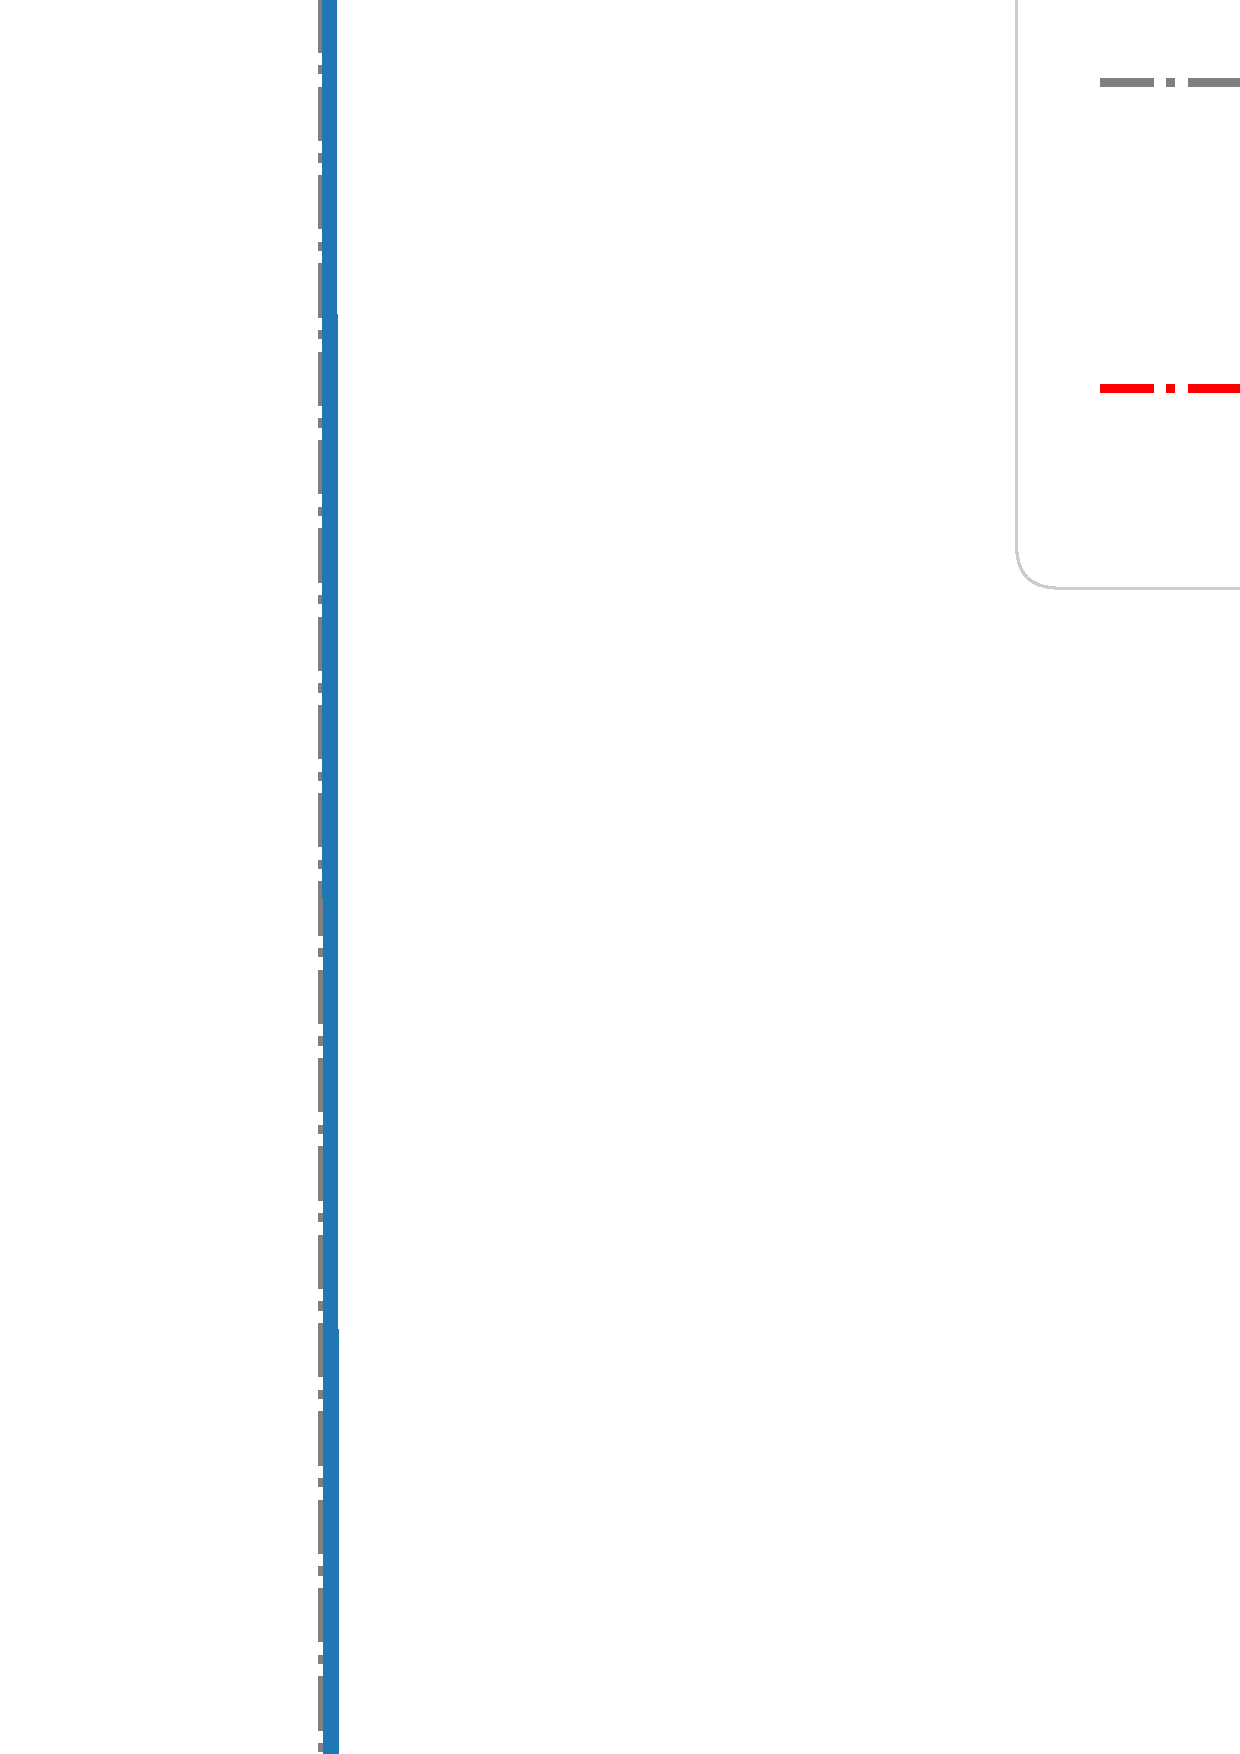
\includegraphics[width=0.45\textwidth]{5GDDoS_Game_plot_purchased_vm_number.pdf}
  \caption{Total Purchased VM v.s. MPO Price}
  \label{fig:VMnum}
\end{figure}

\begin{figure}[!ht]
  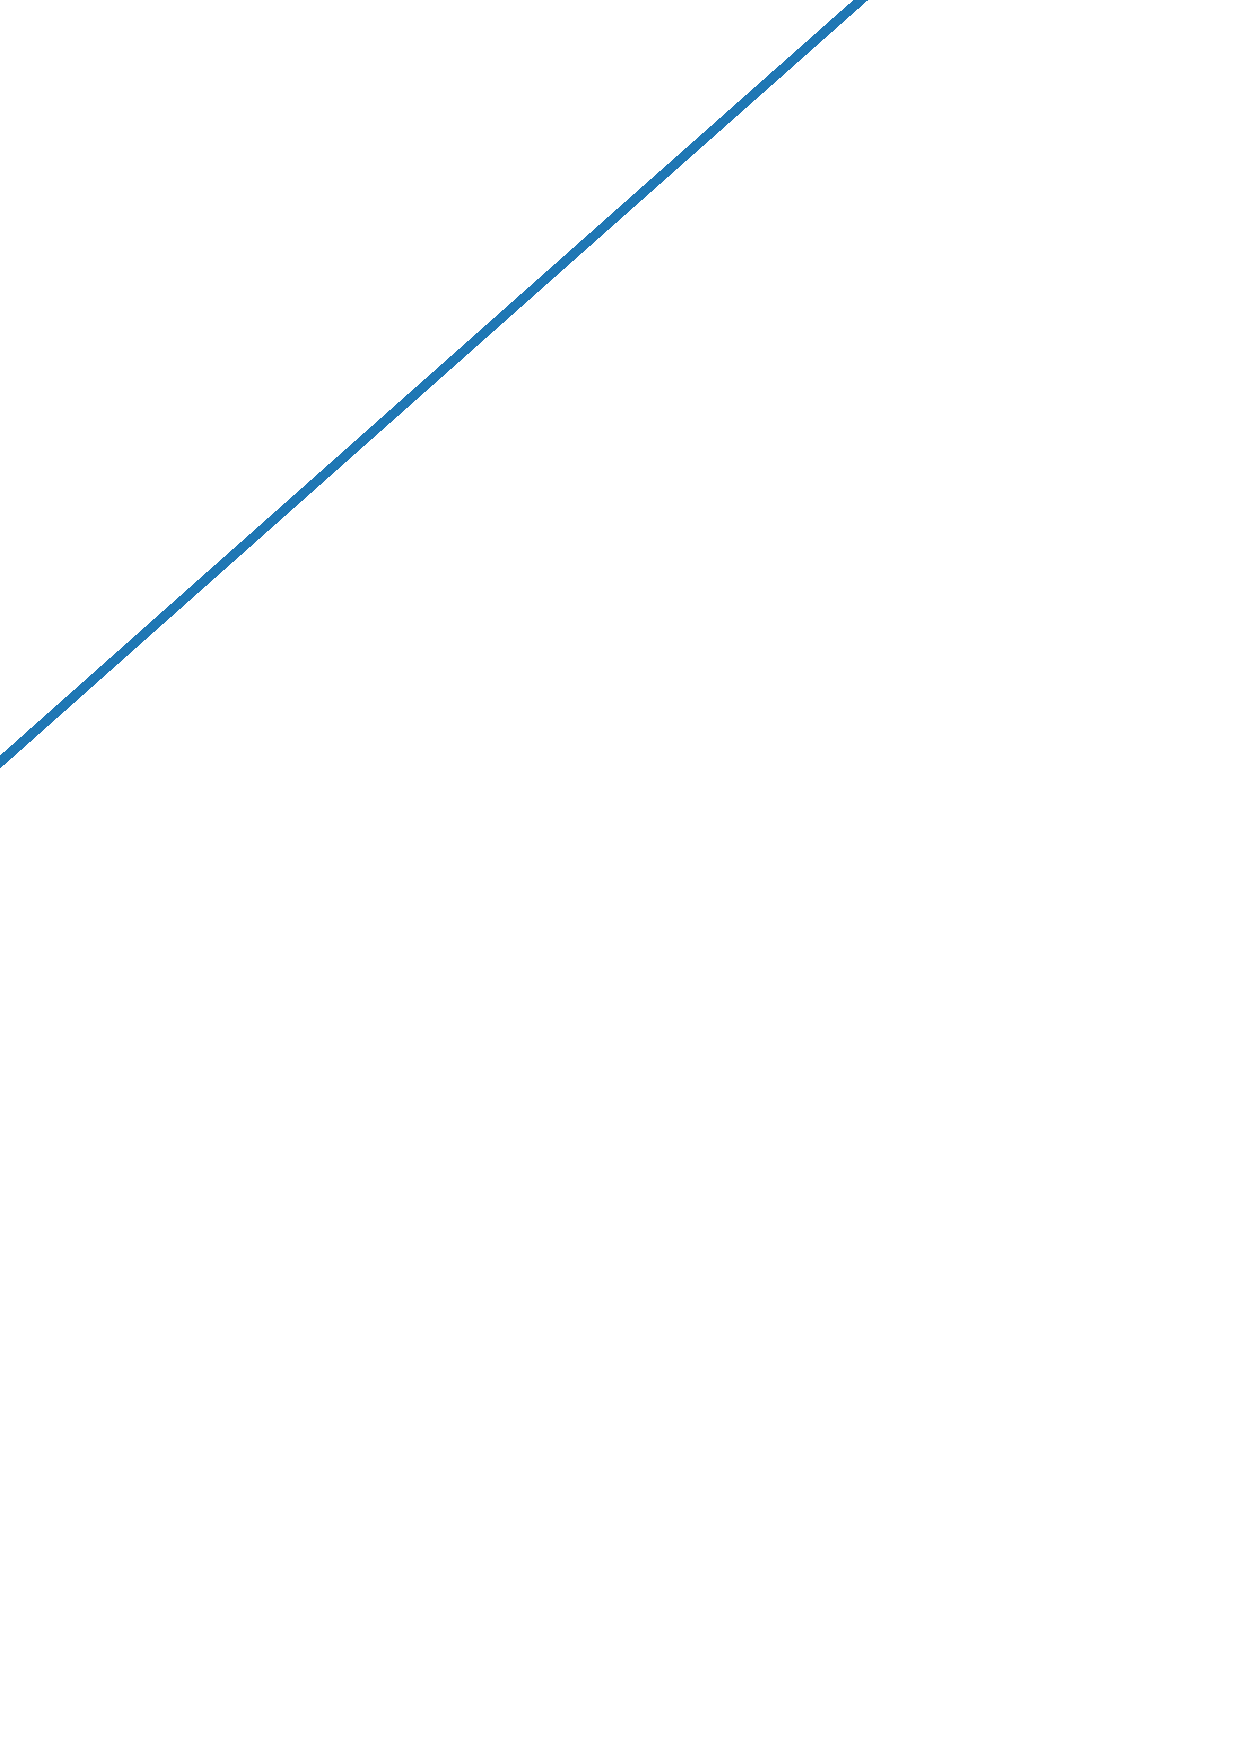
\includegraphics[width=0.45\textwidth]{5GDDoS_Game_plot_MPO_utility.pdf}
\caption{MPO Utility v.s. MPO Price}
\label{fig:MPOutil}
\end{figure}

\subsection{Comparison between different number of end-users scenario}
In reality, the required CPU cycles of the same application are usually similar, so it is necessary to find out the characteristics when deploying different applications on the MEC. In this section, we compare multiple IPS VM deployment schemes on ASPs with various numbers of end-users. Moreover, we discuss two cases: ASP with high workload devices and ASP with low workload devices. In ASP with high workload devices, the required CPU cycles $\chi_{ij}$ is chosen uniformly between $0.8 - 0.9$ Gigacycles. Moreover, the required CPU cycles $\chi_{ij}$ are chosen uniformly between $0.1 - 0.2$ Gigacycles in ASP with low workload devices. We discuss the different characteristics between these two types of ASP in the following. 

% device num high
\begin{figure}[!ht]
  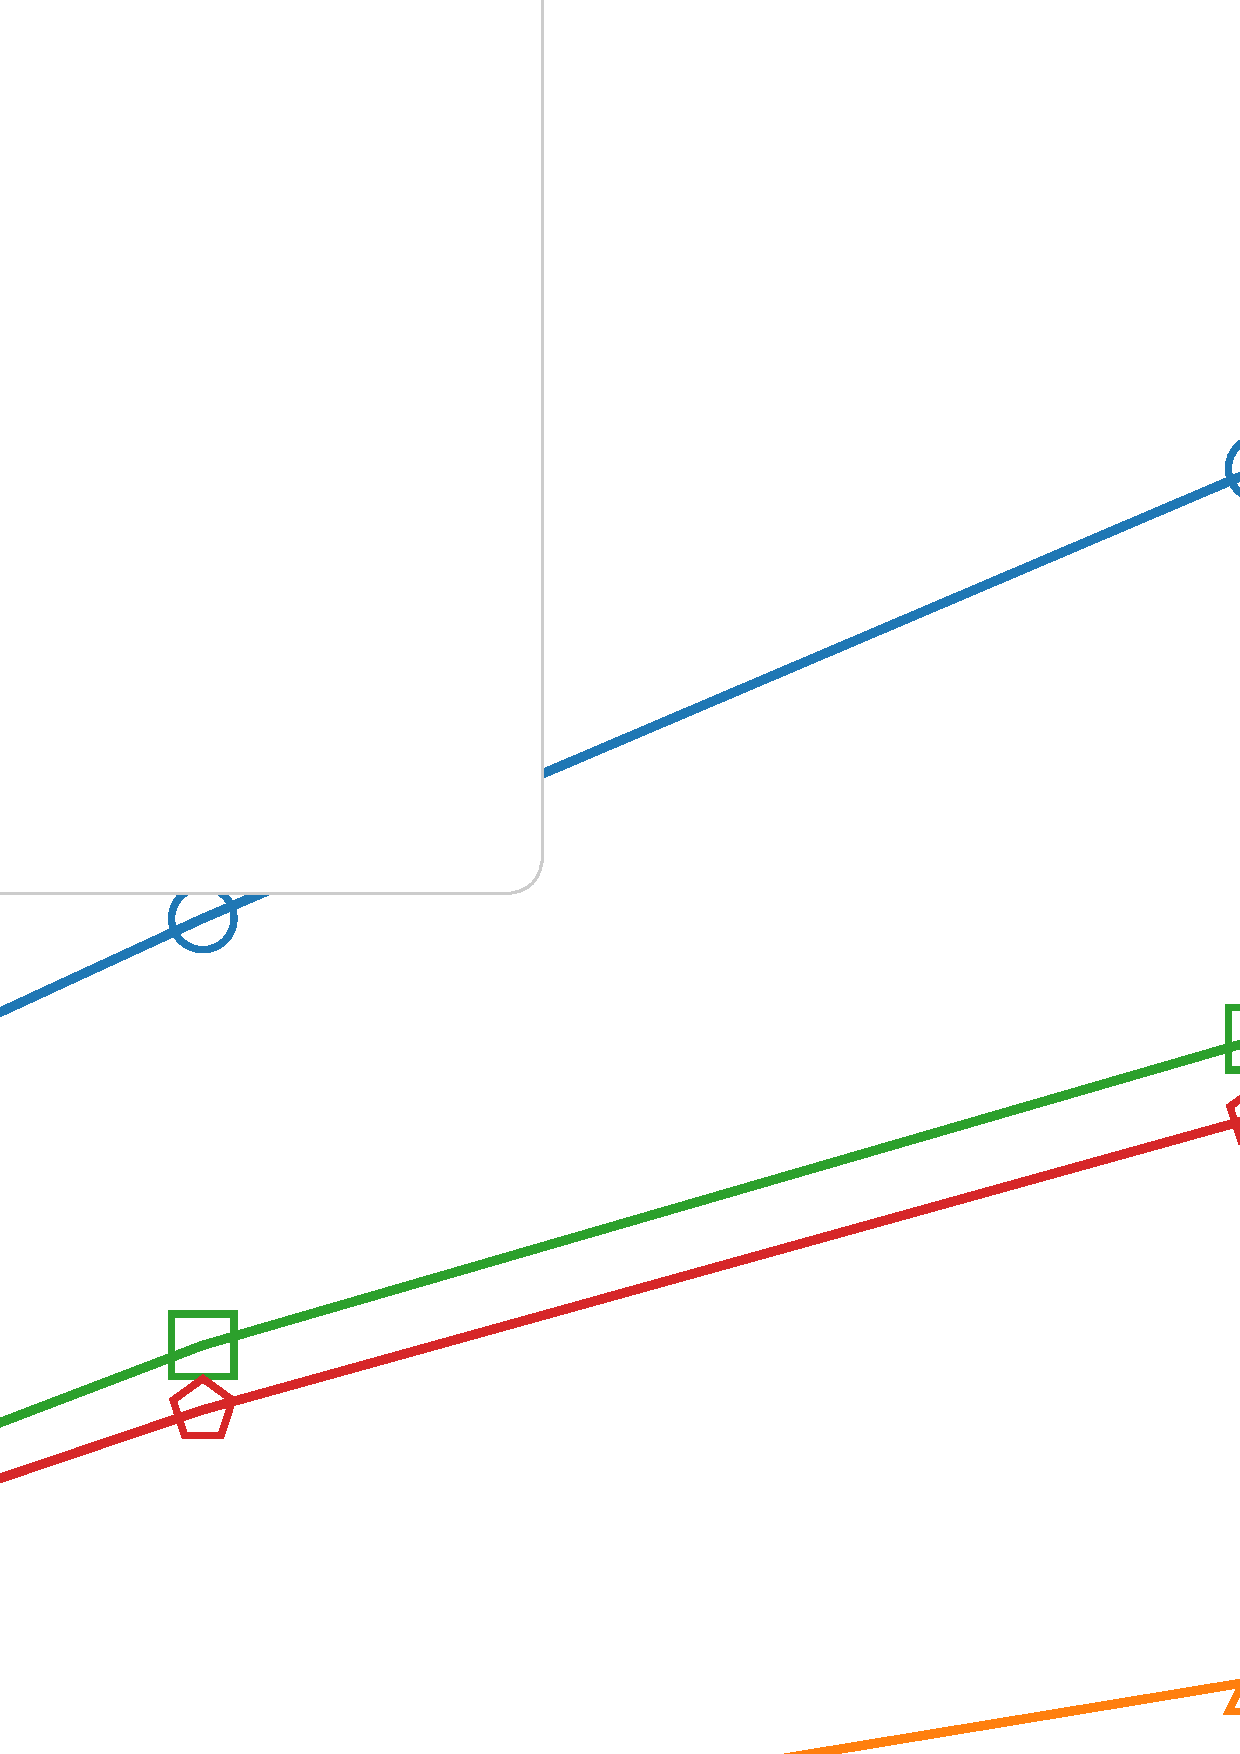
\includegraphics[width=0.45\textwidth]{5GDDoS_Game_social_device_high_cvx.pdf}
    \caption{Social Welfare v.s. Different Number of High Workload End Users}
\label{fig:num_cmp_soc_high}
\end{figure}

\begin{figure}[!ht]
  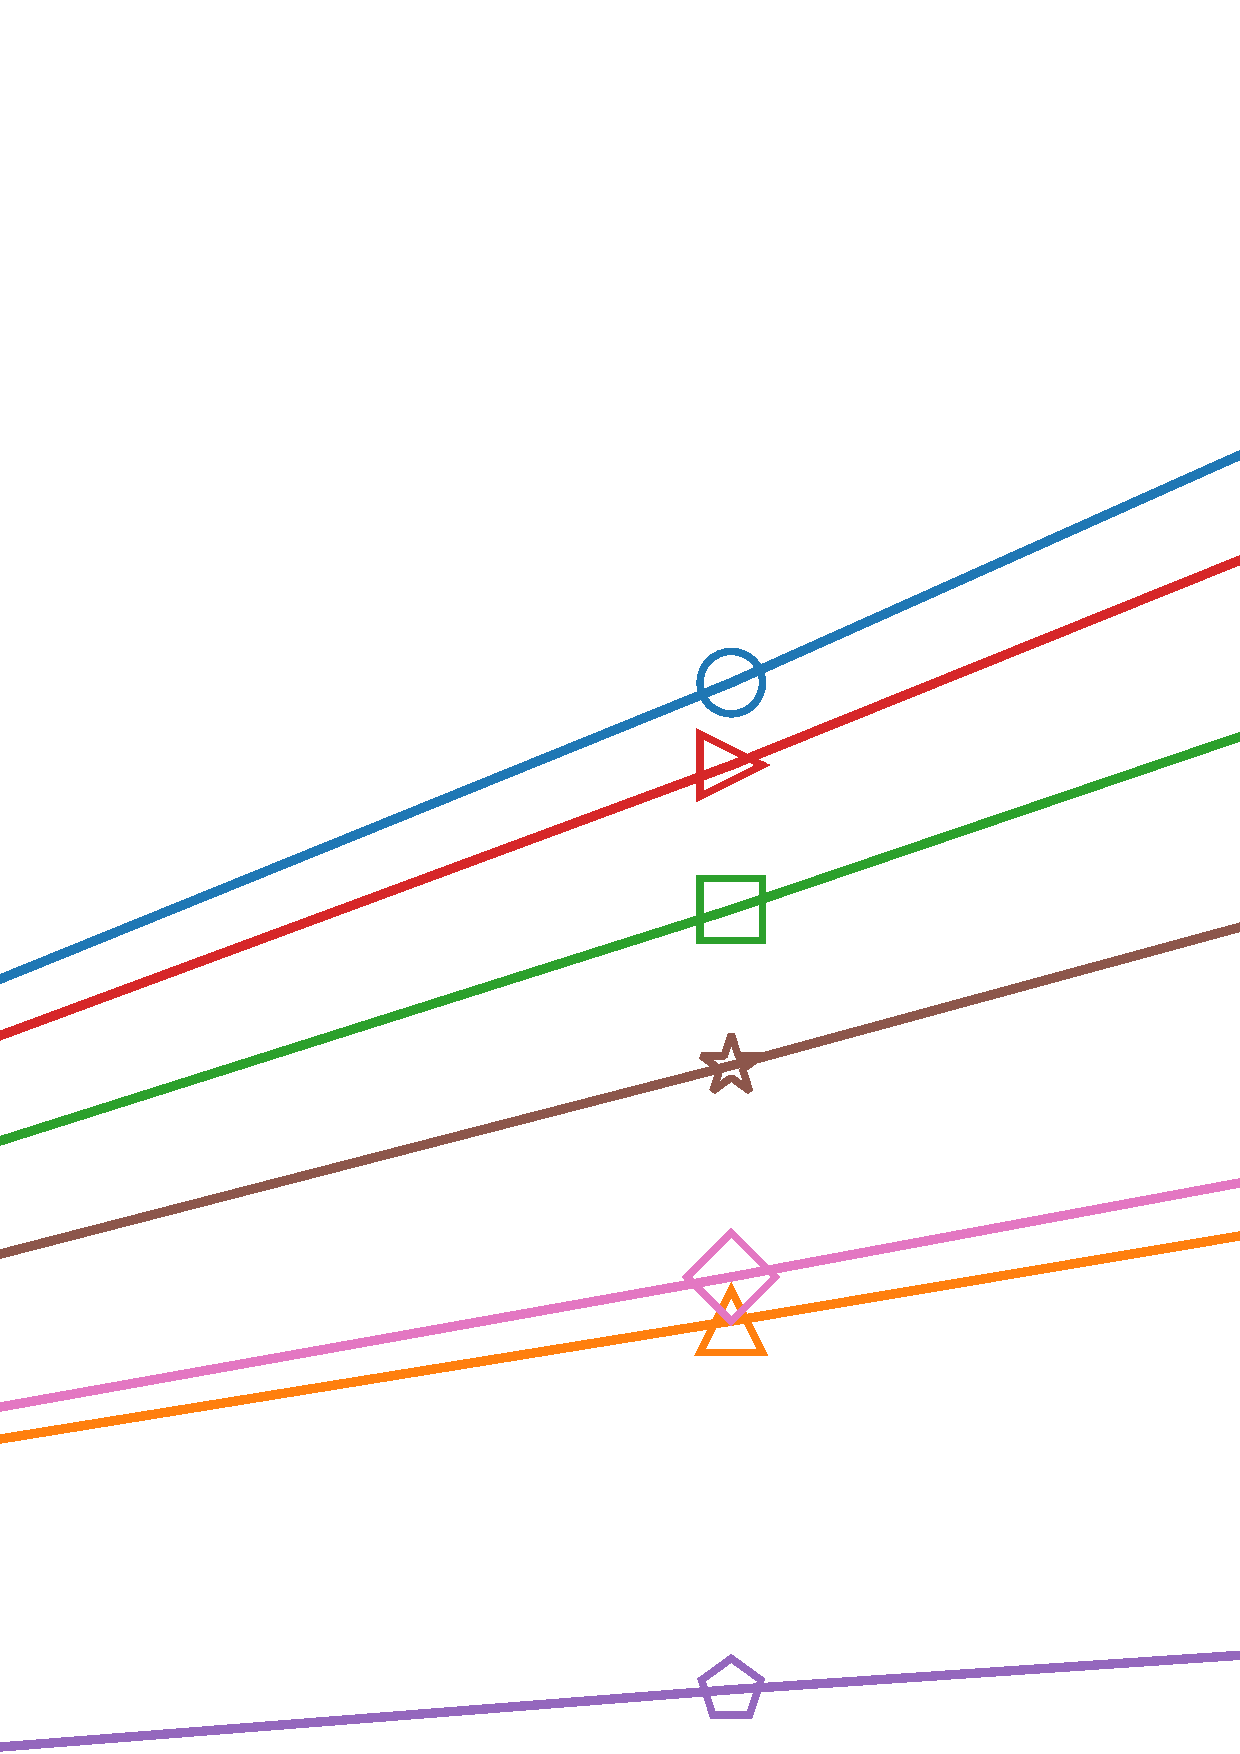
\includegraphics[width=0.45\textwidth]{5GDDoS_Game_asp_device_high_cvx.pdf}
    \caption{ASP Utility v.s. Different Number of High Workload End Users}
\label{fig:num_cmp_asp_high}
\end{figure}

\begin{figure}[!ht]
  \includegraphics[width=0.45\textwidth]{5GDDoS_Game_MPO_device_high_cvx.pdf}
    \caption{MPO Utility v.s. Different Number of High Workload End Users}
\label{fig:num_cmp_mpo_high}
\end{figure}

\textbf{ASP with high workload devices}: 
When considering ASP with high workload devices, by (\ref{eqn:service_rate}), we can find out that because the required CPU cycles are higher, the service rate is lower than the IPS VM efficiency. Thus, the ASP has the incentive to deploy as many VM on IPS services as possible to eradicate malicious requests. In \Cref{fig:num_cmp_asp_high}, our \textit{proposed scheme} has the highest utility. In addition, the \textit{5\% IPS VM} scheme has better utility than \textit{7\% IPS } scheme. The main reason is that the ASP deploys redundant IPS VMs when deploying $7\%$ of their VMs to the IPS service, so the utility of the ASP is lower. Moreover, in \Cref{fig:num_cmp_mpo_high} and \Cref{fig:num_cmp_soc_high} we can discover the same phenomenon. As the number of users increases, the utility of ASPs started to increase because it can serve more users. In addition, the utility of MPO increases because the ASPs buy more VMs from the MPO to serve more users, so the total social welfare increases too.

% device num low
\begin{figure}[!ht]
  \includegraphics[width=0.45\textwidth]{5GDDoS_Game_social_device_low_cvx.pdf}
    \caption{Social Welfare v.s. Different Number of Low Workload End Users}
\label{fig:num_cmp_soc_low}
\end{figure}

\begin{figure}[!ht]
  \includegraphics[width=0.45\textwidth]{5GDDoS_Game_asp_device_low_cvx.pdf}
    \caption{ASP Utility v.s. Different Number of Low Workload End Users}
\label{fig:num_cmp_asp_low}
\end{figure}

\begin{figure}[!ht]
  \includegraphics[width=0.45\textwidth]{5GDDoS_Game_MPO_device_low_cvx.pdf}
    \caption{MPO utility v.s. Different Number of Low Workload End Users}
\label{fig:num_cmp_mpo_low}
\end{figure}

\textbf{ASP with low workload devices}:
When considering ASP with low workload devices, by (\ref{eqn:service_rate}), we can find out that because the required CPU cycles are low, the service rate is higher than the efficiency of IPS VMs. The ASP has more incentive to deploy VMs to serve end-users than to wipe out malicious requests. Because of this characteristic, the ASP has the same behavior as the ASP using the \textit{No IPS} scheme as seen in \Cref{fig:num_cmp_asp_low}. The ASPs' utility in \textit{5\% IPS VM} and \textit{7\% IPS VM} are lower because in this case, it is less efficient to deploy IPS VMs than to deploy VMs to serve users. In addition, our proposed scheme has the highest utility in \Cref{fig:num_cmp_soc_low}, \Cref{fig:num_cmp_asp_low}, and \Cref{fig:num_cmp_mpo_low}.

\subsection{Comparison between different malicious to normal ratio scenario}
In this section, we compare different IPS VM deployment schemes on ASPs with malicious to normal ratio. Similar to the previous section, we discuss two cases: ASP with high workload devices and ASP with low workload devices. The parameters of high and low workload are mentioned in the previous section. We discuss the different characteristics between these two types of ASP in the following. 



% ratio high
\begin{figure}[!ht]
  \includegraphics[width=0.45\textwidth]{5GDDoS_Game_social_ratio_high_cvx.pdf}
    \caption{Different Malicious Users to Total Users Ratio}
\label{fig:ratio_soc_high}
\end{figure}

\begin{figure}[!ht]
  \includegraphics[width=0.45\textwidth]{5GDDoS_Game_asp_ratio_high_cvx.pdf}
    \caption{Different Malicious Users to Total Users Ratio}
\label{fig:ratio_asp_high}
\end{figure}

\begin{figure}[!ht]
  \includegraphics[width=0.45\textwidth]{5GDDoS_Game_MPO_ratio_high_cvx.pdf}
    \caption{Different Malicious Users to Total Users Ratio}
\label{fig:ratio_mpo_high}
\end{figure}

\textbf{ASP with high workload devices}: Similar to the previous, if the ASP has high workload devices, the service rate of the ASP is lower than the efficiency of IPS VMs. As a result, the ASP is more willing to deploy IPS VMs to intercept malicious requests. However, if the ASP deploys too much IPS VMs, it would crowd out VMs serving end-users. In \Cref{fig:ratio_asp_high}, when the malicious users are low, there are fewer malicious requests, and in \textit{7\% IPS VM} scheme, the ASP deploys too much VMs on IPS. Thus the utility is lower. However, when the number of malicious users increases, the \textit{7\% IPS VM} scheme has better utility than the \textit{5\% IPS VM} scheme. Moreover, when the malicious users are low, \textit{Proportional IPS ratio} deploy less IPS VMs, so the utility is lower than \textit{5\% IPS VM}. However, when the number of malicious users increases, the \textit{Proportional IPS ratio} deploys more IPS VMs than \textit{5\% IPS VM} and \textit{7\% IPS VM}, and the ASPs' utility are higher than the scheme mentioned above. In addition, the \textit{Proposed Scheme} has outperformed other schemes in \Cref{fig:ratio_soc_high}, \Cref{fig:ratio_asp_high}, and \Cref{fig:ratio_mpo_high}.

% ratio low
\begin{figure}[!ht]
  \includegraphics[width=0.45\textwidth]{5GDDoS_Game_social_ratio_low_cvx.pdf}
    \caption{Different Malicious Users to Total Users Ratio}
\label{fig:ratio_soc_low}
\end{figure}

\begin{figure}[!ht]
  \includegraphics[width=0.45\textwidth]{5GDDoS_Game_asp_ratio_low_cvx.pdf}
    \caption{Different Malicious Users to Total Users Ratio}
\label{fig:ratio_asp_low}
\end{figure}

\begin{figure}[!ht]
  \includegraphics[width=0.45\textwidth]{5GDDoS_Game_MPO_ratio_low_cvx.pdf}
    \caption{Different Malicious Users to Total Users Ratio}
\label{fig:ratio_mpo_low}
\end{figure}

\textbf{ASP with low workload devices}: Similar to the previous, if the ASP has low workload devices, the service rate of the ASP is higher than efficiency of IPS VMs. As a result, the ASP is more willing to deploy VMs to serve users. So the behaviours of \textit{No IPS} and \textit{Proposed Scheme} is identical. In \Cref{fig:ratio_asp_low}, the \textit{5\% IPS VM} has higher utility than \textit{7\% IPS VM}. In addition, the \textit{Proportional IPS ratio} has deploy lower IPS VMs when the malicious users are low. However, it deploys more IPS VMs when the malicious users are high. When the ratio is $0.3$, it deploys $9\%$ IPS VMs, and the ASPs' utility is lower than \textit{7\% IPS VM} and \textit{5\% IPS VM}. Moreover, the \textit{Proposed Scheme} has outperformed other schemes in \Cref{fig:ratio_soc_low}, \Cref{fig:ratio_asp_low}, and \Cref{fig:ratio_mpo_low}.

\section{Conclusion} \label{sec:conclusion}
In the paper, we proposed a flexible IPS deployment strategy for ASPs to determine the allocation of VM resources for IPS and services to mitigate the expected DDoS attacks. The joint optimization problem of ASP and MPO is formulated as a Stackelberg game to capture the hierarchy relationship. The optimal pricing strategy of MPO and the optimal amount of purchased VM along with the ratio of IPS VM for ASPs are derived. The simulation results verify the effectiveness of the proposed solution in maintaining the service quality and social welfare compared with other baseline schemes.


\bibliographystyle{IEEEtran}
\bibliography{5GDDoS_Game}

\end{document}
